\documentclass[12pt,a4paper]{report}
\usepackage{graphicx,../iman,../extra,../ttbox,../proof,../pdfsetup}

%%\includeonly{}
%%% to index ids: \[\\tt \([a-zA-Z0-9][a-zA-Z0-9_'.]*\)    [\\ttindexbold{\1}
%%% to delete old ones:  \\indexbold{\*[^}]*}
%% run    sedindex ref    to prepare index file
%%% needs chapter on Provers/typedsimp.ML?
\title{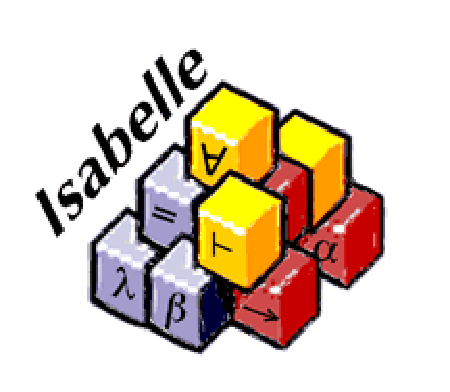
\includegraphics[scale=0.5]{isabelle} \\[4ex] Old Isabelle Reference Manual}

\author{{\em Lawrence C. Paulson}\\
        Computer Laboratory \\ University of Cambridge \\
        \texttt{lcp@cl.cam.ac.uk}\\[3ex] 
        With Contributions by Tobias Nipkow and Markus Wenzel}  

\makeindex

\setcounter{secnumdepth}{2} \setcounter{tocdepth}{2}

\pagestyle{headings}
\sloppy
\binperiod     %%%treat . like a binary operator

\begin{document}
\underscoreoff

\index{definitions|see{rewriting, meta-level}}
\index{rewriting!object-level|see{simplification}}
\index{meta-rules|see{meta-rules}}

\maketitle 
\emph{Note}: this document is part of the earlier Isabelle
documentation and is mostly outdated.  Fully obsolete parts of the
original text have already been removed.  The remaining material
covers some aspects that did not make it into the newer manuals yet.

\subsubsection*{Acknowledgements} 
Tobias Nipkow, of T. U. Munich, wrote most of
  Chapters~\protect\ref{Defining-Logics} and~\protect\ref{chap:simplification}.
  Markus Wenzel contributed to Chapter~\protect\ref{chap:syntax}.
  Jeremy Dawson, Sara Kalvala, Martin
  Simons  and others suggested changes
  and corrections.  The research has been funded by the EPSRC (grants
  GR/G53279, GR/H40570, GR/K57381, GR/K77051, GR/M75440) and by ESPRIT
  (projects 3245: Logical Frameworks, and 6453: Types), and by the DFG
  Schwerpunktprogramm \emph{Deduktion}.

\pagenumbering{roman} \tableofcontents \clearfirst


\chapter{Tactics} \label{tactics}
\index{tactics|(}

\section{Other basic tactics}

\subsection{Inserting premises and facts}\label{cut_facts_tac}
\index{tactics!for inserting facts}\index{assumptions!inserting}
\begin{ttbox} 
cut_facts_tac : thm list -> int -> tactic
\end{ttbox}
These tactics add assumptions to a subgoal.
\begin{ttdescription}
\item[\ttindexbold{cut_facts_tac} {\it thms} {\it i}] 
  adds the {\it thms} as new assumptions to subgoal~$i$.  Once they have
  been inserted as assumptions, they become subject to tactics such as {\tt
    eresolve_tac} and {\tt rewrite_goals_tac}.  Only rules with no premises
  are inserted: Isabelle cannot use assumptions that contain $\Imp$
  or~$\Forall$.  Sometimes the theorems are premises of a rule being
  derived, returned by~{\tt goal}; instead of calling this tactic, you
  could state the goal with an outermost meta-quantifier.

\end{ttdescription}


\subsection{Composition: resolution without lifting}
\index{tactics!for composition}
\begin{ttbox}
compose_tac: (bool * thm * int) -> int -> tactic
\end{ttbox}
{\bf Composing} two rules means resolving them without prior lifting or
renaming of unknowns.  This low-level operation, which underlies the
resolution tactics, may occasionally be useful for special effects.
A typical application is \ttindex{res_inst_tac}, which lifts and instantiates a
rule, then passes the result to {\tt compose_tac}.
\begin{ttdescription}
\item[\ttindexbold{compose_tac} ($flag$, $rule$, $m$) $i$] 
refines subgoal~$i$ using $rule$, without lifting.  The $rule$ is taken to
have the form $\List{\psi@1; \ldots; \psi@m} \Imp \psi$, where $\psi$ need
not be atomic; thus $m$ determines the number of new subgoals.  If
$flag$ is {\tt true} then it performs elim-resolution --- it solves the
first premise of~$rule$ by assumption and deletes that assumption.
\end{ttdescription}


\section{*Managing lots of rules}
These operations are not intended for interactive use.  They are concerned
with the processing of large numbers of rules in automatic proof
strategies.  Higher-order resolution involving a long list of rules is
slow.  Filtering techniques can shorten the list of rules given to
resolution, and can also detect whether a subgoal is too flexible,
with too many rules applicable.

\subsection{Combined resolution and elim-resolution} \label{biresolve_tac}
\index{tactics!resolution}
\begin{ttbox} 
biresolve_tac   : (bool*thm)list -> int -> tactic
bimatch_tac     : (bool*thm)list -> int -> tactic
subgoals_of_brl : bool*thm -> int
lessb           : (bool*thm) * (bool*thm) -> bool
\end{ttbox}
{\bf Bi-resolution} takes a list of $\it (flag,rule)$ pairs.  For each
pair, it applies resolution if the flag is~{\tt false} and
elim-resolution if the flag is~{\tt true}.  A single tactic call handles a
mixture of introduction and elimination rules.

\begin{ttdescription}
\item[\ttindexbold{biresolve_tac} {\it brls} {\it i}] 
refines the proof state by resolution or elim-resolution on each rule, as
indicated by its flag.  It affects subgoal~$i$ of the proof state.

\item[\ttindexbold{bimatch_tac}] 
is like {\tt biresolve_tac}, but performs matching: unknowns in the
proof state are never updated (see~{\S}\ref{match_tac}).

\item[\ttindexbold{subgoals_of_brl}({\it flag},{\it rule})] 
returns the number of new subgoals that bi-res\-o\-lu\-tion would yield for the
pair (if applied to a suitable subgoal).  This is $n$ if the flag is
{\tt false} and $n-1$ if the flag is {\tt true}, where $n$ is the number
of premises of the rule.  Elim-resolution yields one fewer subgoal than
ordinary resolution because it solves the major premise by assumption.

\item[\ttindexbold{lessb} ({\it brl1},{\it brl2})] 
returns the result of 
\begin{ttbox}
subgoals_of_brl{\it brl1} < subgoals_of_brl{\it brl2}
\end{ttbox}
\end{ttdescription}
Note that \hbox{\tt sort lessb {\it brls}} sorts a list of $\it
(flag,rule)$ pairs by the number of new subgoals they will yield.  Thus,
those that yield the fewest subgoals should be tried first.


\subsection{Discrimination nets for fast resolution}\label{filt_resolve_tac}
\index{discrimination nets|bold}
\index{tactics!resolution}
\begin{ttbox} 
net_resolve_tac  : thm list -> int -> tactic
net_match_tac    : thm list -> int -> tactic
net_biresolve_tac: (bool*thm) list -> int -> tactic
net_bimatch_tac  : (bool*thm) list -> int -> tactic
filt_resolve_tac : thm list -> int -> int -> tactic
could_unify      : term*term->bool
filter_thms      : (term*term->bool) -> int*term*thm list -> thm{\ts}list
\end{ttbox}
The module {\tt Net} implements a discrimination net data structure for
fast selection of rules \cite[Chapter 14]{charniak80}.  A term is
classified by the symbol list obtained by flattening it in preorder.
The flattening takes account of function applications, constants, and free
and bound variables; it identifies all unknowns and also regards
\index{lambda abs@$\lambda$-abstractions}
$\lambda$-abstractions as unknowns, since they could $\eta$-contract to
anything.  

A discrimination net serves as a polymorphic dictionary indexed by terms.
The module provides various functions for inserting and removing items from
nets.  It provides functions for returning all items whose term could match
or unify with a target term.  The matching and unification tests are
overly lax (due to the identifications mentioned above) but they serve as
useful filters.

A net can store introduction rules indexed by their conclusion, and
elimination rules indexed by their major premise.  Isabelle provides
several functions for `compiling' long lists of rules into fast
resolution tactics.  When supplied with a list of theorems, these functions
build a discrimination net; the net is used when the tactic is applied to a
goal.  To avoid repeatedly constructing the nets, use currying: bind the
resulting tactics to \ML{} identifiers.

\begin{ttdescription}
\item[\ttindexbold{net_resolve_tac} {\it thms}] 
builds a discrimination net to obtain the effect of a similar call to {\tt
resolve_tac}.

\item[\ttindexbold{net_match_tac} {\it thms}] 
builds a discrimination net to obtain the effect of a similar call to {\tt
match_tac}.

\item[\ttindexbold{net_biresolve_tac} {\it brls}] 
builds a discrimination net to obtain the effect of a similar call to {\tt
biresolve_tac}.

\item[\ttindexbold{net_bimatch_tac} {\it brls}] 
builds a discrimination net to obtain the effect of a similar call to {\tt
bimatch_tac}.

\item[\ttindexbold{filt_resolve_tac} {\it thms} {\it maxr} {\it i}] 
uses discrimination nets to extract the {\it thms} that are applicable to
subgoal~$i$.  If more than {\it maxr\/} theorems are applicable then the
tactic fails.  Otherwise it calls {\tt resolve_tac}.  

This tactic helps avoid runaway instantiation of unknowns, for example in
type inference.

\item[\ttindexbold{could_unify} ({\it t},{\it u})] 
returns {\tt false} if~$t$ and~$u$ are `obviously' non-unifiable, and
otherwise returns~{\tt true}.  It assumes all variables are distinct,
reporting that {\tt ?a=?a} may unify with {\tt 0=1}.

\item[\ttindexbold{filter_thms} $could\; (limit,prem,thms)$] 
returns the list of potentially resolvable rules (in {\it thms\/}) for the
subgoal {\it prem}, using the predicate {\it could\/} to compare the
conclusion of the subgoal with the conclusion of each rule.  The resulting list
is no longer than {\it limit}.
\end{ttdescription}

\index{tactics|)}


%%% Local Variables: 
%%% mode: latex
%%% TeX-master: "ref"
%%% End: 


\chapter{Theorems and Forward Proof}
\index{theorems|(}

Theorems, which represent the axioms, theorems and rules of
object-logics, have type \mltydx{thm}.  This chapter describes
operations that join theorems in forward proof.  Most theorem
operations are intended for advanced applications, such as programming
new proof procedures.


\section{Basic operations on theorems}

\subsection{Expanding definitions in theorems}
\index{meta-rewriting!in theorems}
\begin{ttbox} 
rewrite_rule       : thm list -> thm -> thm
rewrite_goals_rule : thm list -> thm -> thm
\end{ttbox}
\begin{ttdescription}
\item[\ttindexbold{rewrite_rule} {\it defs} {\it thm}]  
unfolds the {\it defs} throughout the theorem~{\it thm}.

\item[\ttindexbold{rewrite_goals_rule} {\it defs} {\it thm}]  
unfolds the {\it defs} in the premises of~{\it thm}, but it leaves the
conclusion unchanged.  This rule is the basis for \ttindex{rewrite_goals_tac},
but it serves little purpose in forward proof.
\end{ttdescription}


\subsection{Instantiating unknowns in a theorem} \label{sec:instantiate}
\index{instantiation}
\begin{alltt}\footnotesize
read_instantiate    :                (string*string) list -> thm -> thm
read_instantiate_sg :     Sign.sg -> (string*string) list -> thm -> thm
cterm_instantiate   :                  (cterm*cterm) list -> thm -> thm
instantiate'      : ctyp option list -> cterm option list -> thm -> thm
\end{alltt}
These meta-rules instantiate type and term unknowns in a theorem.  They are
occasionally useful.  They can prevent difficulties with higher-order
unification, and define specialized versions of rules.
\begin{ttdescription}
\item[\ttindexbold{read_instantiate} {\it insts} {\it thm}] 
processes the instantiations {\it insts} and instantiates the rule~{\it
thm}.  The processing of instantiations is described
in \S\ref{res_inst_tac}, under {\tt res_inst_tac}.  

Use {\tt res_inst_tac}, not {\tt read_instantiate}, to instantiate a rule
and refine a particular subgoal.  The tactic allows instantiation by the
subgoal's parameters, and reads the instantiations using the signature
associated with the proof state.

Use {\tt read_instantiate_sg} below if {\it insts\/} appears to be treated
incorrectly.

\item[\ttindexbold{read_instantiate_sg} {\it sg} {\it insts} {\it thm}]
  is like \texttt{read_instantiate {\it insts}~{\it thm}}, but it reads
  the instantiations under signature~{\it sg}.  This is necessary to
  instantiate a rule from a general theory, such as first-order logic,
  using the notation of some specialized theory.  Use the function {\tt
    sign_of} to get a theory's signature.

\item[\ttindexbold{cterm_instantiate} {\it ctpairs} {\it thm}] 
is similar to {\tt read_instantiate}, but the instantiations are provided
as pairs of certified terms, not as strings to be read.

\item[\ttindexbold{instantiate'} {\it ctyps} {\it cterms} {\it thm}]
  instantiates {\it thm} according to the positional arguments {\it
    ctyps} and {\it cterms}.  Counting from left to right, schematic
  variables $?x$ are either replaced by $t$ for any argument
  \texttt{Some\(\;t\)}, or left unchanged in case of \texttt{None} or
  if the end of the argument list is encountered.  Types are
  instantiated before terms.

\end{ttdescription}


\subsection{Miscellaneous forward rules}\label{MiscellaneousForwardRules}
\index{theorems!standardizing}
\begin{ttbox} 
standard         :               thm -> thm
zero_var_indexes :               thm -> thm
make_elim        :               thm -> thm
rule_by_tactic   :     tactic -> thm -> thm
rotate_prems     :        int -> thm -> thm
permute_prems    : int -> int -> thm -> thm
rearrange_prems  :   int list -> thm -> thm
\end{ttbox}
\begin{ttdescription}
\item[\ttindexbold{standard} $thm$] puts $thm$ into the standard form
  of object-rules.  It discharges all meta-assumptions, replaces free
  variables by schematic variables, renames schematic variables to
  have subscript zero, also strips outer (meta) quantifiers and
  removes dangling sort hypotheses.

\item[\ttindexbold{zero_var_indexes} $thm$] 
makes all schematic variables have subscript zero, renaming them to avoid
clashes. 

\item[\ttindexbold{make_elim} $thm$] 
\index{rules!converting destruction to elimination}
converts $thm$, which should be  a destruction rule of the form
$\List{P@1;\ldots;P@m}\Imp 
Q$, to the elimination rule $\List{P@1; \ldots; P@m; Q\Imp R}\Imp R$.  This
is the basis for destruct-resolution: {\tt dresolve_tac}, etc.

\item[\ttindexbold{rule_by_tactic} {\it tac} {\it thm}] 
  applies {\it tac\/} to the {\it thm}, freezing its variables first, then
  yields the proof state returned by the tactic.  In typical usage, the
  {\it thm\/} represents an instance of a rule with several premises, some
  with contradictory assumptions (because of the instantiation).  The
  tactic proves those subgoals and does whatever else it can, and returns
  whatever is left.
  
\item[\ttindexbold{rotate_prems} $k$ $thm$] rotates the premises of $thm$ to
  the left by~$k$ positions (to the right if $k<0$).  It simply calls
  \texttt{permute_prems}, below, with $j=0$.  Used with
  \texttt{eresolve_tac}\index{*eresolve_tac!on other than first premise}, it
  gives the effect of applying the tactic to some other premise of $thm$ than
  the first.

\item[\ttindexbold{permute_prems} $j$ $k$ $thm$] rotates the premises of $thm$
  leaving the first $j$ premises unchanged.  It
  requires $0\leq j\leq n$, where $n$ is the number of premises.  If $k$ is
  positive then it rotates the remaining $n-j$ premises to the left; if $k$ is
  negative then it rotates the premises to the right.

\item[\ttindexbold{rearrange_prems} $ps$ $thm$] permutes the premises of $thm$
   where the value at the $i$-th position (counting from $0$) in the list $ps$
   gives the position within the original thm to be transferred to position $i$.
   Any remaining trailing positions are left unchanged.
\end{ttdescription}


\subsection{Taking a theorem apart}
\index{theorems!taking apart}
\index{flex-flex constraints}
\begin{ttbox} 
cprop_of      : thm -> cterm
concl_of      : thm -> term
prems_of      : thm -> term list
cprems_of     : thm -> cterm list
nprems_of     : thm -> int
tpairs_of     : thm -> (term*term) list
theory_of_thm : thm -> theory
dest_state : thm * int -> (term*term) list * term list * term * term
\end{ttbox}
\begin{ttdescription}
\item[\ttindexbold{cprop_of} $thm$] returns the statement of $thm$ as
  a certified term.
  
\item[\ttindexbold{concl_of} $thm$] returns the conclusion of $thm$ as
  a term.
  
\item[\ttindexbold{prems_of} $thm$] returns the premises of $thm$ as a
  list of terms.
  
\item[\ttindexbold{cprems_of} $thm$] returns the premises of $thm$ as
  a list of certified terms.

\item[\ttindexbold{nprems_of} $thm$] 
returns the number of premises in $thm$, and is equivalent to {\tt
  length~(prems_of~$thm$)}.

\item[\ttindexbold{tpairs_of} $thm$] returns the flex-flex constraints
  of $thm$.
  
\item[\ttindexbold{theory_of_thm} $thm$] returns the theory associated
  with $thm$.  Note that this does a lookup in Isabelle's global
  database of loaded theories.

\item[\ttindexbold{dest_state} $(thm,i)$] 
decomposes $thm$ as a tuple containing a list of flex-flex constraints, a
list of the subgoals~1 to~$i-1$, subgoal~$i$, and the rest of the theorem
(this will be an implication if there are more than $i$ subgoals).

\end{ttdescription}


\subsection{*Sort hypotheses} \label{sec:sort-hyps}
\index{sort hypotheses}
\begin{ttbox} 
strip_shyps         : thm -> thm
strip_shyps_warning : thm -> thm
\end{ttbox}

Isabelle's type variables are decorated with sorts, constraining them to
certain ranges of types.  This has little impact when sorts only serve for
syntactic classification of types --- for example, FOL distinguishes between
terms and other types.  But when type classes are introduced through axioms,
this may result in some sorts becoming {\em empty\/}: where one cannot exhibit
a type belonging to it because certain sets of axioms are unsatisfiable.

If a theorem contains a type variable that is constrained by an empty
sort, then that theorem has no instances.  It is basically an instance
of {\em ex falso quodlibet}.  But what if it is used to prove another
theorem that no longer involves that sort?  The latter theorem holds
only if under an additional non-emptiness assumption.

Therefore, Isabelle's theorems carry around sort hypotheses.  The {\tt
shyps} field is a list of sorts occurring in type variables in the current
{\tt prop} and {\tt hyps} fields.  It may also includes sorts used in the
theorem's proof that no longer appear in the {\tt prop} or {\tt hyps}
fields --- so-called {\em dangling\/} sort constraints.  These are the
critical ones, asserting non-emptiness of the corresponding sorts.
 
Isabelle automatically removes extraneous sorts from the {\tt shyps} field at
the end of a proof, provided that non-emptiness can be established by looking
at the theorem's signature: from the {\tt classes} and {\tt arities}
information.  This operation is performed by \texttt{strip_shyps} and
\texttt{strip_shyps_warning}.

\begin{ttdescription}
  
\item[\ttindexbold{strip_shyps} $thm$] removes any extraneous sort hypotheses
  that can be witnessed from the type signature.
  
\item[\ttindexbold{strip_shyps_warning}] is like \texttt{strip_shyps}, but
  issues a warning message of any pending sort hypotheses that do not have a
  (syntactic) witness.

\end{ttdescription}


\subsection{Tracing flags for unification}
\index{tracing!of unification}
\begin{ttbox} 
Unify.trace_simp   : bool ref \hfill\textbf{initially false}
Unify.trace_types  : bool ref \hfill\textbf{initially false}
Unify.trace_bound  : int ref \hfill\textbf{initially 10}
Unify.search_bound : int ref \hfill\textbf{initially 20}
\end{ttbox}
Tracing the search may be useful when higher-order unification behaves
unexpectedly.  Letting {\tt res_inst_tac} circumvent the problem is easier,
though.
\begin{ttdescription}
\item[set Unify.trace_simp;] 
causes tracing of the simplification phase.

\item[set Unify.trace_types;] 
generates warnings of incompleteness, when unification is not considering
all possible instantiations of type unknowns.

\item[Unify.trace_bound := $n$;] 
causes unification to print tracing information once it reaches depth~$n$.
Use $n=0$ for full tracing.  At the default value of~10, tracing
information is almost never printed.

\item[Unify.search_bound := $n$;] prevents unification from
  searching past the depth~$n$.  Because of this bound, higher-order
  unification cannot return an infinite sequence, though it can return
  an exponentially long one.  The search rarely approaches the default value
  of~20.  If the search is cut off, unification prints a warning
  \texttt{Unification bound exceeded}.
\end{ttdescription}


\section{*Primitive meta-level inference rules}
\index{meta-rules|(}

\subsection{Logical equivalence rules}
\index{meta-equality}
\begin{ttbox} 
equal_intr : thm -> thm -> thm 
equal_elim : thm -> thm -> thm
\end{ttbox}
\begin{ttdescription}
\item[\ttindexbold{equal_intr} $thm@1$ $thm@2$] 
applies $({\equiv}I)$ to $thm@1$ and~$thm@2$.  It maps the premises~$\psi$
and~$\phi$ to the conclusion~$\phi\equiv\psi$; the assumptions are those of
the first premise with~$\phi$ removed, plus those of
the second premise with~$\psi$ removed.

\item[\ttindexbold{equal_elim} $thm@1$ $thm@2$] 
applies $({\equiv}E)$ to $thm@1$ and~$thm@2$.  It maps the premises
$\phi\equiv\psi$ and $\phi$ to the conclusion~$\psi$.
\end{ttdescription}


\subsection{Equality rules}
\index{meta-equality}
\begin{ttbox} 
reflexive  : cterm -> thm
symmetric  : thm -> thm
transitive : thm -> thm -> thm
\end{ttbox}
\begin{ttdescription}
\item[\ttindexbold{reflexive} $ct$] 
makes the theorem \(ct\equiv ct\). 

\item[\ttindexbold{symmetric} $thm$] 
maps the premise $a\equiv b$ to the conclusion $b\equiv a$.

\item[\ttindexbold{transitive} $thm@1$ $thm@2$] 
maps the premises $a\equiv b$ and $b\equiv c$ to the conclusion~${a\equiv c}$.
\end{ttdescription}


\subsection{The $\lambda$-conversion rules}
\index{lambda calc@$\lambda$-calculus}
\begin{ttbox} 
beta_conversion : cterm -> thm
extensional     : thm -> thm
abstract_rule   : string -> cterm -> thm -> thm
combination     : thm -> thm -> thm
\end{ttbox} 
There is no rule for $\alpha$-conversion because Isabelle regards
$\alpha$-convertible theorems as equal.
\begin{ttdescription}
\item[\ttindexbold{beta_conversion} $ct$] 
makes the theorem $((\lambda x.a)(b)) \equiv a[b/x]$, where $ct$ is the
term $(\lambda x.a)(b)$.

\item[\ttindexbold{extensional} $thm$] 
maps the premise $f(x) \equiv g(x)$ to the conclusion $f\equiv g$.
Parameter~$x$ is taken from the premise.  It may be an unknown or a free
variable (provided it does not occur in the assumptions); it must not occur
in $f$ or~$g$.

\item[\ttindexbold{abstract_rule} $v$ $x$ $thm$] 
maps the premise $a\equiv b$ to the conclusion $(\lambda x.a) \equiv
(\lambda x.b)$, abstracting over all occurrences (if any!) of~$x$.
Parameter~$x$ is supplied as a cterm.  It may be an unknown or a free
variable (provided it does not occur in the assumptions).  In the
conclusion, the bound variable is named~$v$.

\item[\ttindexbold{combination} $thm@1$ $thm@2$] 
maps the premises $f\equiv g$ and $a\equiv b$ to the conclusion~$f(a)\equiv
g(b)$.
\end{ttdescription}


\section{Derived rules for goal-directed proof}
Most of these rules have the sole purpose of implementing particular
tactics.  There are few occasions for applying them directly to a theorem.

\subsection{Resolution}
\index{resolution}
\begin{ttbox} 
biresolution : bool -> (bool*thm)list -> int -> thm
               -> thm Seq.seq
\end{ttbox}
\begin{ttdescription}
\item[\ttindexbold{biresolution} $match$ $rules$ $i$ $state$] 
performs bi-resolution on subgoal~$i$ of $state$, using the list of $\it
(flag,rule)$ pairs.  For each pair, it applies resolution if the flag
is~{\tt false} and elim-resolution if the flag is~{\tt true}.  If $match$
is~{\tt true}, the $state$ is not instantiated.
\end{ttdescription}


\subsection{Composition: resolution without lifting}
\index{resolution!without lifting}
\begin{ttbox}
compose   : thm * int * thm -> thm list
COMP      : thm * thm -> thm
bicompose : bool -> bool * thm * int -> int -> thm
            -> thm Seq.seq
\end{ttbox}
In forward proof, a typical use of composition is to regard an assertion of
the form $\phi\Imp\psi$ as atomic.  Schematic variables are not renamed, so
beware of clashes!
\begin{ttdescription}
\item[\ttindexbold{compose} ($thm@1$, $i$, $thm@2$)] 
uses $thm@1$, regarded as an atomic formula, to solve premise~$i$
of~$thm@2$.  Let $thm@1$ and $thm@2$ be $\psi$ and $\List{\phi@1; \ldots;
\phi@n} \Imp \phi$.  For each $s$ that unifies~$\psi$ and $\phi@i$, the
result list contains the theorem
\[ (\List{\phi@1; \ldots; \phi@{i-1}; \phi@{i+1}; \ldots; \phi@n} \Imp \phi)s.
\]

\item[$thm@1$ \ttindexbold{COMP} $thm@2$] 
calls \hbox{\tt compose ($thm@1$, 1, $thm@2$)} and returns the result, if
unique; otherwise, it raises exception~\xdx{THM}\@.  It is
analogous to {\tt RS}\@.  

For example, suppose that $thm@1$ is $a=b\Imp b=a$, a symmetry rule, and
that $thm@2$ is $\List{P\Imp Q; \neg Q} \Imp\neg P$, which is the
principle of contrapositives.  Then the result would be the
derived rule $\neg(b=a)\Imp\neg(a=b)$.

\item[\ttindexbold{bicompose} $match$ ($flag$, $rule$, $m$) $i$ $state$]
refines subgoal~$i$ of $state$ using $rule$, without lifting.  The $rule$
is taken to have the form $\List{\psi@1; \ldots; \psi@m} \Imp \psi$, where
$\psi$ need not be atomic; thus $m$ determines the number of new
subgoals.  If $flag$ is {\tt true} then it performs elim-resolution --- it
solves the first premise of~$rule$ by assumption and deletes that
assumption.  If $match$ is~{\tt true}, the $state$ is not instantiated.
\end{ttdescription}


\subsection{Other meta-rules}
\begin{ttbox} 
rename_params_rule : string list * int -> thm -> thm
\end{ttbox}
\begin{ttdescription}

\item[\ttindexbold{rename_params_rule} ({\it names}, {\it i}) $thm$] 
uses the $names$ to rename the parameters of premise~$i$ of $thm$.  The
names must be distinct.  If there are fewer names than parameters, then the
rule renames the innermost parameters and may modify the remaining ones to
ensure that all the parameters are distinct.
\index{parameters!renaming}

\end{ttdescription}
\index{meta-rules|)}


\section{Proof terms}\label{sec:proofObjects}
\index{proof terms|(} Isabelle can record the full meta-level proof of each
theorem.  The proof term contains all logical inferences in detail.
%while
%omitting bookkeeping steps that have no logical meaning to an outside
%observer.  Rewriting steps are recorded in similar detail as the output of
%simplifier tracing. 
Resolution and rewriting steps are broken down to primitive rules of the
meta-logic. The proof term can be inspected by a separate proof-checker,
for example.

According to the well-known {\em Curry-Howard isomorphism}, a proof can
be viewed as a $\lambda$-term. Following this idea, proofs
in Isabelle are internally represented by a datatype similar to the one for
terms described in \S\ref{sec:terms}.
\begin{ttbox}
infix 8 % %%;

datatype proof =
   PBound of int
 | Abst of string * typ option * proof
 | AbsP of string * term option * proof
 | op % of proof * term option
 | op %% of proof * proof
 | Hyp of term
 | PThm of (string * (string * string list) list) *
           proof * term * typ list option
 | PAxm of string * term * typ list option
 | Oracle of string * term * typ list option
 | MinProof of proof list;
\end{ttbox}

\begin{ttdescription}
\item[\ttindexbold{Abst} ($a$, $\tau$, $prf$)] is the abstraction over
a {\it term variable} of type $\tau$ in the body $prf$. Logically, this
corresponds to $\bigwedge$ introduction. The name $a$ is used only for
parsing and printing.
\item[\ttindexbold{AbsP} ($a$, $\varphi$, $prf$)] is the abstraction
over a {\it proof variable} standing for a proof of proposition $\varphi$
in the body $prf$. This corresponds to $\Longrightarrow$ introduction.
\item[$prf$ \% $t$] \index{\%@{\tt\%}|bold}
is the application of proof $prf$ to term $t$
which corresponds to $\bigwedge$ elimination.
\item[$prf@1$ \%\% $prf@2$] \index{\%\%@{\tt\%\%}|bold}
is the application of proof $prf@1$ to
proof $prf@2$ which corresponds to $\Longrightarrow$ elimination.
\item[\ttindexbold{PBound} $i$] is a {\em proof variable} with de Bruijn
\cite{debruijn72} index $i$.
\item[\ttindexbold{Hyp} $\varphi$] corresponds to the use of a meta level
hypothesis $\varphi$.
\item[\ttindexbold{PThm} (($name$, $tags$), $prf$, $\varphi$, $\overline{\tau}$)]
stands for a pre-proved theorem, where $name$ is the name of the theorem,
$prf$ is its actual proof, $\varphi$ is the proven proposition,
and $\overline{\tau}$ is
a type assignment for the type variables occurring in the proposition.
\item[\ttindexbold{PAxm} ($name$, $\varphi$, $\overline{\tau}$)]
corresponds to the use of an axiom with name $name$ and proposition
$\varphi$, where $\overline{\tau}$ is a type assignment for the type
variables occurring in the proposition.
\item[\ttindexbold{Oracle} ($name$, $\varphi$, $\overline{\tau}$)]
denotes the invocation of an oracle with name $name$ which produced
a proposition $\varphi$, where $\overline{\tau}$ is a type assignment
for the type variables occurring in the proposition.
\item[\ttindexbold{MinProof} $prfs$]
represents a {\em minimal proof} where $prfs$ is a list of theorems,
axioms or oracles.
\end{ttdescription}
Note that there are no separate constructors
for abstraction and application on the level of {\em types}, since
instantiation of type variables is accomplished via the type assignments
attached to {\tt Thm}, {\tt Axm} and {\tt Oracle}.

Each theorem's derivation is stored as the {\tt der} field of its internal
record: 
\begin{ttbox} 
#2 (#der (rep_thm conjI));
{\out PThm (("HOL.conjI", []),}
{\out   AbsP ("H", None, AbsP ("H", None, \dots)), \dots, None) %}
{\out     None % None : Proofterm.proof}
\end{ttbox}
This proof term identifies a labelled theorem, {\tt conjI} of theory
\texttt{HOL}, whose underlying proof is
{\tt AbsP ("H", None, AbsP ("H", None, $\dots$))}. 
The theorem is applied to two (implicit) term arguments, which correspond
to the two variables occurring in its proposition.

Isabelle's inference kernel can produce proof objects with different
levels of detail. This is controlled via the global reference variable
\ttindexbold{proofs}:
\begin{ttdescription}
\item[proofs := 0;] only record uses of oracles
\item[proofs := 1;] record uses of oracles as well as dependencies
  on other theorems and axioms
\item[proofs := 2;] record inferences in full detail
\end{ttdescription}
Reconstruction and checking of proofs as described in \S\ref{sec:reconstruct_proofs}
will not work for proofs constructed with {\tt proofs} set to
{\tt 0} or {\tt 1}.
Theorems involving oracles will be printed with a
suffixed \verb|[!]| to point out the different quality of confidence achieved.

\medskip

The dependencies of theorems can be viewed using the function
\ttindexbold{thm_deps}\index{theorems!dependencies}:
\begin{ttbox}
thm_deps [\(thm@1\), \(\ldots\), \(thm@n\)];
\end{ttbox}
generates the dependency graph of the theorems $thm@1$, $\ldots$, $thm@n$ and
displays it using Isabelle's graph browser. For this to work properly,
the theorems in question have to be proved with {\tt proofs} set to a value
greater than {\tt 0}. You can use
\begin{ttbox}
ThmDeps.enable : unit -> unit
ThmDeps.disable : unit -> unit
\end{ttbox}
to set \texttt{proofs} appropriately.

\subsection{Reconstructing and checking proof terms}\label{sec:reconstruct_proofs}
\index{proof terms!reconstructing}
\index{proof terms!checking}

When looking at the above datatype of proofs more closely, one notices that
some arguments of constructors are {\it optional}. The reason for this is that
keeping a full proof term for each theorem would result in enormous memory
requirements. Fortunately, typical proof terms usually contain quite a lot of
redundant information that can be reconstructed from the context. Therefore,
Isabelle's inference kernel creates only {\em partial} (or {\em implicit})
\index{proof terms!partial} proof terms, in which
all typing information in terms, all term and type labels of abstractions
{\tt AbsP} and {\tt Abst}, and (if possible) some argument terms of
\verb!%! are omitted. The following functions are available for
reconstructing and checking proof terms:
\begin{ttbox}
Reconstruct.reconstruct_proof :
  Sign.sg -> term -> Proofterm.proof -> Proofterm.proof
Reconstruct.expand_proof :
  Sign.sg -> string list -> Proofterm.proof -> Proofterm.proof
ProofChecker.thm_of_proof : theory -> Proofterm.proof -> thm
\end{ttbox}

\begin{ttdescription}
\item[Reconstruct.reconstruct_proof $sg$ $t$ $prf$]
turns the partial proof $prf$ into a full proof of the
proposition denoted by $t$, with respect to signature $sg$.
Reconstruction will fail with an error message if $prf$
is not a proof of $t$, is ill-formed, or does not contain
sufficient information for reconstruction by
{\em higher order pattern unification}
\cite{nipkow-patterns, Berghofer-Nipkow:2000:TPHOL}.
The latter may only happen for proofs
built up ``by hand'' but not for those produced automatically
by Isabelle's inference kernel.
\item[Reconstruct.expand_proof $sg$
  \ttlbrack$name@1$, $\ldots$, $name@n${\ttrbrack} $prf$]
expands and reconstructs the proofs of all theorems with names
$name@1$, $\ldots$, $name@n$ in the (full) proof $prf$.
\item[ProofChecker.thm_of_proof $thy$ $prf$] turns the (full) proof
$prf$ into a theorem with respect to theory $thy$ by replaying
it using only primitive rules from Isabelle's inference kernel.
\end{ttdescription}

\subsection{Parsing and printing proof terms}
\index{proof terms!parsing}
\index{proof terms!printing}

Isabelle offers several functions for parsing and printing
proof terms. The concrete syntax for proof terms is described
in Fig.\ts\ref{fig:proof_gram}.
Implicit term arguments in partial proofs are indicated
by ``{\tt _}''.
Type arguments for theorems and axioms may be specified using
\verb!%! or ``$\cdot$'' with an argument of the form {\tt TYPE($type$)}
(see \S\ref{sec:basic_syntax}).
They must appear before any other term argument of a theorem
or axiom. In contrast to term arguments, type arguments may
be completely omitted.
\begin{ttbox}
ProofSyntax.read_proof : theory -> bool -> string -> Proofterm.proof
ProofSyntax.pretty_proof : Sign.sg -> Proofterm.proof -> Pretty.T
ProofSyntax.pretty_proof_of : bool -> thm -> Pretty.T
ProofSyntax.print_proof_of : bool -> thm -> unit
\end{ttbox}
\begin{figure}
\begin{center}
\begin{tabular}{rcl}
$proof$  & $=$ & {\tt Lam} $params${\tt .} $proof$ ~~$|$~~
                 $\Lambda params${\tt .} $proof$ \\
         & $|$ & $proof$ \verb!%! $any$ ~~$|$~~
                 $proof$ $\cdot$ $any$ \\
         & $|$ & $proof$ \verb!%%! $proof$ ~~$|$~~
                 $proof$ {\boldmath$\cdot$} $proof$ \\
         & $|$ & $id$ ~~$|$~~ $longid$ \\\\
$param$  & $=$ & $idt$ ~~$|$~~ $idt$ {\tt :} $prop$ ~~$|$~~
                 {\tt (} $param$ {\tt )} \\\\
$params$ & $=$ & $param$ ~~$|$~~ $param$ $params$
\end{tabular}
\end{center}
\caption{Proof term syntax}\label{fig:proof_gram}
\end{figure}
The function {\tt read_proof} reads in a proof term with
respect to a given theory. The boolean flag indicates whether
the proof term to be parsed contains explicit typing information
to be taken into account.
Usually, typing information is left implicit and
is inferred during proof reconstruction. The pretty printing
functions operating on theorems take a boolean flag as an
argument which indicates whether the proof term should
be reconstructed before printing.

The following example (based on Isabelle/HOL) illustrates how
to parse and check proof terms. We start by parsing a partial
proof term
\begin{ttbox}
val prf = ProofSyntax.read_proof Main.thy false
  "impI % _ % _ %% (Lam H : _. conjE % _ % _ % _ %% H %%
     (Lam (H1 : _) H2 : _. conjI % _ % _ %% H2 %% H1))";
{\out val prf = PThm (("HOL.impI", []), \dots, \dots, None) % None % None %%}
{\out   AbsP ("H", None, PThm (("HOL.conjE", []), \dots, \dots, None) %}
{\out     None % None % None %% PBound 0 %%}
{\out     AbsP ("H1", None, AbsP ("H2", None, \dots))) : Proofterm.proof}
\end{ttbox}
The statement to be established by this proof is
\begin{ttbox}
val t = term_of
  (read_cterm (sign_of Main.thy) ("A & B --> B & A", propT));
{\out val t = Const ("Trueprop", "bool => prop") $}
{\out   (Const ("op -->", "[bool, bool] => bool") $}
{\out     \dots $ \dots : Term.term}
\end{ttbox}
Using {\tt t} we can reconstruct the full proof
\begin{ttbox}
val prf' = Reconstruct.reconstruct_proof (sign_of Main.thy) t prf;
{\out val prf' = PThm (("HOL.impI", []), \dots, \dots, Some []) %}
{\out   Some (Const ("op &", \dots) $ Free ("A", \dots) $ Free ("B", \dots)) %}
{\out   Some (Const ("op &", \dots) $ Free ("B", \dots) $ Free ("A", \dots)) %%}
{\out   AbsP ("H", Some (Const ("Trueprop", \dots) $ \dots), \dots)}
{\out     : Proofterm.proof}
\end{ttbox}
This proof can finally be turned into a theorem
\begin{ttbox}
val thm = ProofChecker.thm_of_proof Main.thy prf';
{\out val thm = "A & B --> B & A" : Thm.thm}
\end{ttbox}

\index{proof terms|)}
\index{theorems|)}


%%% Local Variables: 
%%% mode: latex
%%% TeX-master: "ref"
%%% End: 


\chapter{Defining Logics} \label{Defining-Logics}

\section{Mixfix declarations} \label{sec:mixfix}
\index{mixfix declarations|(}

When defining a theory, you declare new constants by giving their names,
their type, and an optional {\bf mixfix annotation}.  Mixfix annotations
allow you to extend Isabelle's basic $\lambda$-calculus syntax with
readable notation.  They can express any context-free priority grammar.
Isabelle syntax definitions are inspired by \OBJ~\cite{OBJ}; they are more
general than the priority declarations of \ML\ and Prolog.

A mixfix annotation defines a production of the priority grammar.  It
describes the concrete syntax, the translation to abstract syntax, and the
pretty printing.  Special case annotations provide a simple means of
specifying infix operators and binders.

\subsection{The general mixfix form}
Here is a detailed account of mixfix declarations.  Suppose the following
line occurs within a {\tt consts} or {\tt syntax} section of a {\tt .thy}
file:
\begin{center}
  {\tt $c$ ::\ "$\sigma$" ("$template$" $ps$ $p$)}
\end{center}
This constant declaration and mixfix annotation are interpreted as follows:
\begin{itemize}\index{productions}
\item The string {\tt $c$} is the name of the constant associated with the
  production; unless it is a valid identifier, it must be enclosed in
  quotes.  If $c$ is empty (given as~{\tt ""}) then this is a copy
  production.\index{productions!copy} Otherwise, parsing an instance of the
  phrase $template$ generates the \AST{} {\tt ("$c$" $a@1$ $\ldots$
    $a@n$)}, where $a@i$ is the \AST{} generated by parsing the $i$-th
  argument.

  \item The constant $c$, if non-empty, is declared to have type $\sigma$
    ({\tt consts} section only).

  \item The string $template$ specifies the right-hand side of
    the production.  It has the form
    \[ w@0 \;_\; w@1 \;_\; \ldots \;_\; w@n, \]
    where each occurrence of {\tt_} denotes an argument position and
    the~$w@i$ do not contain~{\tt _}.  (If you want a literal~{\tt _} in
    the concrete syntax, you must escape it as described below.)  The $w@i$
    may consist of \rmindex{delimiters}, spaces or
    \rmindex{pretty printing} annotations (see below).

  \item The type $\sigma$ specifies the production's nonterminal symbols
    (or name tokens).  If $template$ is of the form above then $\sigma$
    must be a function type with at least~$n$ argument positions, say
    $\sigma = [\tau@1, \dots, \tau@n] \To \tau$.  Nonterminal symbols are
    derived from the types $\tau@1$, \ldots,~$\tau@n$, $\tau$ as described
    below.  Any of these may be function types.

  \item The optional list~$ps$ may contain at most $n$ integers, say {\tt
      [$p@1$, $\ldots$, $p@m$]}, where $p@i$ is the minimal
    priority\indexbold{priorities} required of any phrase that may appear
    as the $i$-th argument.  Missing priorities default to~0.
    
  \item The integer $p$ is the priority of this production.  If
    omitted, it defaults to the maximal priority.  Priorities range
    between 0 and \ttindexbold{max_pri} (= 1000).

\end{itemize}
%
The resulting production is \[ A^{(p)}= w@0\, A@1^{(p@1)}\, w@1\,
A@2^{(p@2)}\, \dots\, A@n^{(p@n)}\, w@n \] where $A$ and the $A@i$ are the
nonterminals corresponding to the types $\tau$ and $\tau@i$ respectively.
The nonterminal symbol associated with a type $(\ldots)ty$ is {\tt logic}, if
this is a logical type (namely one of class {\tt logic} excluding {\tt
prop}).  Otherwise it is $ty$ (note that only the outermost type constructor
is taken into account).  Finally, the nonterminal of a type variable is {\tt
any}.

\begin{warn}
  Theories must sometimes declare types for purely syntactic purposes ---
  merely playing the role of nonterminals.  One example is \tydx{type}, the
  built-in type of types.  This is a `type of all types' in the syntactic
  sense only.  Do not declare such types under {\tt arities} as belonging to
  class {\tt logic}\index{*logic class}, for that would make them useless as
  separate nonterminal symbols.
\end{warn}

Associating nonterminals with types allows a constant's type to specify
syntax as well.  We can declare the function~$f$ to have type $[\tau@1,
\ldots, \tau@n]\To \tau$ and, through a mixfix annotation, specify the layout
of the function's $n$ arguments.  The constant's name, in this case~$f$, will
also serve as the label in the abstract syntax tree.

You may also declare mixfix syntax without adding constants to the theory's
signature, by using a {\tt syntax} section instead of {\tt consts}.  Thus a
production need not map directly to a logical function (this typically
requires additional syntactic translations, see also
Chapter~\ref{chap:syntax}).


\medskip
As a special case of the general mixfix declaration, the form
\begin{center}
  {\tt $c$ ::\ "$\sigma$" ("$template$")}
\end{center}
specifies no priorities.  The resulting production puts no priority
constraints on any of its arguments and has maximal priority itself.
Omitting priorities in this manner is prone to syntactic ambiguities unless
the production's right-hand side is fully bracketed, as in
\verb|"if _ then _ else _ fi"|.

Omitting the mixfix annotation completely, as in {\tt $c$ ::\ "$\sigma$"},
is sensible only if~$c$ is an identifier.  Otherwise you will be unable to
write terms involving~$c$.


\subsection{Example: arithmetic expressions}
\index{examples!of mixfix declarations}
This theory specification contains a {\tt syntax} section with mixfix
declarations encoding the priority grammar from
\S\ref{sec:priority_grammars}:
\begin{ttbox}
ExpSyntax = Pure +
types
  exp
syntax
  "0" :: exp                 ("0"      9)
  "+" :: [exp, exp] => exp   ("_ + _"  [0, 1] 0)
  "*" :: [exp, exp] => exp   ("_ * _"  [3, 2] 2)
  "-" :: exp => exp          ("- _"    [3] 3)
end
\end{ttbox}
Executing {\tt Syntax.print_gram} reveals the productions derived from the
above mixfix declarations (lots of additional information deleted):
\begin{ttbox}
Syntax.print_gram (syn_of ExpSyntax.thy);
{\out exp = "0"  => "0" (9)}
{\out exp = exp[0] "+" exp[1]  => "+" (0)}
{\out exp = exp[3] "*" exp[2]  => "*" (2)}
{\out exp = "-" exp[3]  => "-" (3)}
\end{ttbox}

Note that because {\tt exp} is not of class {\tt logic}, it has been
retained as a separate nonterminal.  This also entails that the syntax
does not provide for identifiers or paranthesized expressions.
Normally you would also want to add the declaration {\tt arities
  exp::logic} after {\tt types} and use {\tt consts} instead of {\tt
  syntax}.  Try this as an exercise and study the changes in the
grammar.


\subsection{Infixes}
\indexbold{infixes}

Infix operators associating to the left or right can be declared using
{\tt infixl} or {\tt infixr}.  Basically, the form {\tt $c$ ::\ 
  $\sigma$ (infixl $p$)} abbreviates the mixfix declarations
\begin{ttbox}
"op \(c\)" :: \(\sigma\)   ("(_ \(c\)/ _)" [\(p\), \(p+1\)] \(p\))
"op \(c\)" :: \(\sigma\)   ("op \(c\)")
\end{ttbox}
and {\tt $c$ ::\ $\sigma$ (infixr $p$)} abbreviates the mixfix declarations
\begin{ttbox}
"op \(c\)" :: \(\sigma\)   ("(_ \(c\)/ _)" [\(p+1\), \(p\)] \(p\))
"op \(c\)" :: \(\sigma\)   ("op \(c\)")
\end{ttbox}
The infix operator is declared as a constant with the prefix {\tt op}.
Thus, prefixing infixes with \sdx{op} makes them behave like ordinary
function symbols, as in \ML.  Special characters occurring in~$c$ must be
escaped, as in delimiters, using a single quote.

A slightly more general form of infix declarations allows constant
names to be independent from their concrete syntax, namely \texttt{$c$
  ::\ $\sigma$\ (infixl "$sy$" $p$)}, the same for \texttt{infixr}.  As
an example consider:
\begin{ttbox}
and :: [bool, bool] => bool  (infixr "&" 35)
\end{ttbox}
The internal constant name will then be just \texttt{and}, without any
\texttt{op} prefixed.


\subsection{Binders}
\indexbold{binders}
\begingroup
\def\Q{{\cal Q}}
A {\bf binder} is a variable-binding construct such as a quantifier.  The
constant declaration
\begin{ttbox}
\(c\) :: \(\sigma\)   (binder "\(\Q\)" [\(pb\)] \(p\))
\end{ttbox}
introduces a constant~$c$ of type~$\sigma$, which must have the form
$(\tau@1 \To \tau@2) \To \tau@3$.  Its concrete syntax is $\Q~x.P$, where
$x$ is a bound variable of type~$\tau@1$, the body~$P$ has type $\tau@2$
and the whole term has type~$\tau@3$.  The optional integer $pb$
specifies the body's priority, by default~$p$.  Special characters
in $\Q$ must be escaped using a single quote.

The declaration is expanded internally to something like
\begin{ttbox}
\(c\)\hskip3pt    :: (\(\tau@1\) => \(\tau@2\)) => \(\tau@3\)
"\(\Q\)"  :: [idts, \(\tau@2\)] => \(\tau@3\)   ("(3\(\Q\)_./ _)" [0, \(pb\)] \(p\))
\end{ttbox}
Here \ndx{idts} is the nonterminal symbol for a list of identifiers with
\index{type constraints}
optional type constraints (see Fig.\ts\ref{fig:pure_gram}).  The
declaration also installs a parse translation\index{translations!parse}
for~$\Q$ and a print translation\index{translations!print} for~$c$ to
translate between the internal and external forms.

A binder of type $(\sigma \To \tau) \To \tau$ can be nested by giving a
list of variables.  The external form $\Q~x@1~x@2 \ldots x@n. P$
corresponds to the internal form
\[ c(\lambda x@1. c(\lambda x@2. \ldots c(\lambda x@n. P) \ldots)). \]

\medskip
For example, let us declare the quantifier~$\forall$:\index{quantifiers}
\begin{ttbox}
All :: ('a => o) => o   (binder "ALL " 10)
\end{ttbox}
This lets us write $\forall x.P$ as either {\tt All(\%$x$.$P$)} or {\tt ALL
  $x$.$P$}.  When printing, Isabelle prefers the latter form, but must fall
back on ${\tt All}(P)$ if $P$ is not an abstraction.  Both $P$ and {\tt ALL
  $x$.$P$} have type~$o$, the type of formulae, while the bound variable
can be polymorphic.
\endgroup

\index{mixfix declarations|)}


\section{*Alternative print modes} \label{sec:prmodes}
\index{print modes|(}
%
Isabelle's pretty printer supports alternative output syntaxes.  These
may be used independently or in cooperation.  The currently active
print modes (with precedence from left to right) are determined by a
reference variable.
\begin{ttbox}\index{*print_mode}
print_mode: string list ref
\end{ttbox}
Initially this may already contain some print mode identifiers,
depending on how Isabelle has been invoked (e.g.\ by some user
interface).  So changes should be incremental --- adding or deleting
modes relative to the current value.

Any \ML{} string is a legal print mode identifier, without any predeclaration
required.  The following names should be considered reserved, though:
\texttt{""} (the empty string), \texttt{symbols}, \texttt{xsymbols}, and
\texttt{latex}.

There is a separate table of mixfix productions for pretty printing
associated with each print mode.  The currently active ones are
conceptually just concatenated from left to right, with the standard
syntax output table always coming last as default.  Thus mixfix
productions of preceding modes in the list may override those of later
ones.

\medskip The canonical application of print modes is optional printing
of mathematical symbols from a special screen font instead of {\sc
  ascii}.  Another example is to re-use Isabelle's advanced
$\lambda$-term printing mechanisms to generate completely different
output, say for interfacing external tools like \rmindex{model
  checkers} (see also \texttt{HOL/Modelcheck}).

\index{print modes|)}


\section{Ambiguity of parsed expressions} \label{sec:ambiguity}
\index{ambiguity!of parsed expressions}

To keep the grammar small and allow common productions to be shared
all logical types (except {\tt prop}) are internally represented
by one nonterminal, namely {\tt logic}.  This and omitted or too freely
chosen priorities may lead to ways of parsing an expression that were
not intended by the theory's maker.  In most cases Isabelle is able to
select one of multiple parse trees that an expression has lead
to by checking which of them can be typed correctly.  But this may not
work in every case and always slows down parsing.
The warning and error messages that can be produced during this process are
as follows:

If an ambiguity can be resolved by type inference the following
warning is shown to remind the user that parsing is (unnecessarily)
slowed down.  In cases where it's not easily possible to eliminate the
ambiguity the frequency of the warning can be controlled by changing
the value of {\tt Syntax.ambiguity_level} which has type {\tt int
ref}.  Its default value is 1 and by increasing it one can control how
many parse trees are necessary to generate the warning.

\begin{ttbox}
{\out Ambiguous input "\dots"}
{\out produces the following parse trees:}
{\out \dots}
{\out Fortunately, only one parse tree is type correct.}
{\out You may still want to disambiguate your grammar or your input.}
\end{ttbox}

The following message is normally caused by using the same
syntax in two different productions:

\begin{ttbox}
{\out Ambiguous input "..."}
{\out produces the following parse trees:}
{\out \dots}
{\out More than one term is type correct:}
{\out \dots}
\end{ttbox}

Ambiguities occuring in syntax translation rules cannot be resolved by
type inference because it is not necessary for these rules to be type
correct.  Therefore Isabelle always generates an error message and the
ambiguity should be eliminated by changing the grammar or the rule.


%%% Local Variables: 
%%% mode: latex
%%% TeX-master: "ref"
%%% End: 


\chapter{Isar document syntax}

\section{Inner versus outer syntax}

\section{Lexical matters}

\section{Common syntax entities}

\subsection{Atoms}

\begin{rail}
  name : ident | symident | string
  ;

  nameref : name | longident
  ;

  text : nameref | verbatim
  ;
\end{rail}

\subsection{Comments}

\begin{rail}
  comment : (() | '--' text)
  ;
  interest : (() | '\%')
  ;
\end{rail}


\subsection{Sorts and arities}

\begin{rail}
  sort : nameref | lbrace (nameref * ',') rbrace
  ;
  arity : ( () | '(' (sort + ',') ')' ) sort
  ;
  simple\-arity : ( () | '(' (sort + ',') ')' ) nameref
  ;
\end{rail}


\subsection{Terms and Types}

\begin{rail}
  
\end{rail}

\subsection{Mixfix annotations}


\subsection{}

\subsection{}

\subsection{}


%%% Local Variables: 
%%% mode: latex
%%% TeX-master: "isar-ref"
%%% End: 

%% $Id$
\chapter{Substitution Tactics} \label{substitution}
\index{tactics!substitution|(}\index{equality|(}

Replacing equals by equals is a basic form of reasoning.  Isabelle supports
several kinds of equality reasoning.  {\bf Substitution} means to replace
free occurrences of~$t$ by~$u$ in a subgoal.  This is easily done, given an
equality $t=u$, provided the logic possesses the appropriate rule ---
unless you want to substitute even in the assumptions.  The tactic
{\tt hyp_subst_tac} performs substitution in the assumptions, but it
works via object-level implication, and therefore must be specially set up
for each suitable object-logic.

Substitution should not be confused with object-level {\bf rewriting}.
Given equalities of the form $t=u$, rewriting replaces instances of~$t$ by
corresponding instances of~$u$, and continues until it reaches a normal
form.  Substitution handles `one-off' replacements by particular
equalities, while rewriting handles general equalities.
Chapter~\ref{simp-chap} discusses Isabelle's rewriting tactics.


\section{Substitution rules}
\index{substitution!rules}\index{*subst theorem}
Many logics include a substitution rule of the form
$$ \List{\Var{a}=\Var{b}; \Var{P}(\Var{a})} \Imp 
   \Var{P}(\Var{b})  \eqno(subst)$$
In backward proof, this may seem difficult to use: the conclusion
$\Var{P}(\Var{b})$ admits far too many unifiers.  But, if the theorem {\tt
eqth} asserts $t=u$, then \hbox{\tt eqth RS subst} is the derived rule
\[ \Var{P}(t) \Imp \Var{P}(u). \]
Provided $u$ is not an unknown, resolution with this rule is
well-behaved.\footnote{Unifying $\Var{P}(u)$ with a formula~$Q$
expresses~$Q$ in terms of its dependence upon~$u$.  There are still $2^k$
unifiers, if $Q$ has $k$ occurrences of~$u$, but Isabelle ensures that
the first unifier includes all the occurrences.}  To replace $u$ by~$t$ in
subgoal~$i$, use
\begin{ttbox} 
resolve_tac [eqth RS subst] \(i\) {\it.}
\end{ttbox}
To replace $t$ by~$u$ in
subgoal~$i$, use
\begin{ttbox} 
resolve_tac [eqth RS ssubst] \(i\) {\it,}
\end{ttbox}
where \tdxbold{ssubst} is the `swapped' substitution rule
$$ \List{\Var{a}=\Var{b}; \Var{P}(\Var{b})} \Imp 
   \Var{P}(\Var{a}).  \eqno(ssubst)$$
If \tdx{sym} denotes the symmetry rule
\(\Var{a}=\Var{b}\Imp\Var{b}=\Var{a}\), then {\tt ssubst} is just
\hbox{\tt sym RS subst}.  Many logics with equality include the rules {\tt
subst} and {\tt ssubst}, as well as {\tt refl}, {\tt sym} and {\tt trans}
(for the usual equality laws).  Examples include {\tt FOL} and {\tt HOL},
but not {\tt CTT} (Constructive Type Theory).

Elim-resolution is well-behaved with assumptions of the form $t=u$.
To replace $u$ by~$t$ or $t$ by~$u$ in subgoal~$i$, use
\begin{ttbox} 
eresolve_tac [subst] \(i\)    {\it or}    eresolve_tac [ssubst] \(i\) {\it.}
\end{ttbox}


\section{Substitution in the hypotheses}
\index{assumptions!substitution in}
Substitution rules, like other rules of natural deduction, do not affect
the assumptions.  This can be inconvenient.  Consider proving the subgoal
\[ \List{c=a; c=b} \Imp a=b. \]
Calling {\tt eresolve_tac\ts[ssubst]\ts\(i\)} simply discards the
assumption~$c=a$, since $c$ does not occur in~$a=b$.  Of course, we can
work out a solution.  First apply {\tt eresolve_tac\ts[subst]\ts\(i\)},
replacing~$a$ by~$c$:
\[ \List{c=b} \Imp c=b \]
Equality reasoning can be difficult, but this trivial proof requires
nothing more sophisticated than substitution in the assumptions.
Object-logics that include the rule~$(subst)$ provide tactics for this
purpose:
\begin{ttbox} 
hyp_subst_tac       : int -> tactic
bound_hyp_subst_tac : int -> tactic
\end{ttbox}
\begin{ttdescription}
\item[\ttindexbold{hyp_subst_tac} {\it i}] 
  selects an equality assumption of the form $t=u$ or $u=t$, where $t$ is a
  free variable or parameter.  Deleting this assumption, it replaces $t$
  by~$u$ throughout subgoal~$i$, including the other assumptions.

\item[\ttindexbold{bound_hyp_subst_tac} {\it i}] 
  is similar but only substitutes for parameters (bound variables).
  Uses for this are discussed below.
\end{ttdescription}
The term being replaced must be a free variable or parameter.  Substitution
for constants is usually unhelpful, since they may appear in other
theorems.  For instance, the best way to use the assumption $0=1$ is to
contradict a theorem that states $0\not=1$, rather than to replace 0 by~1
in the subgoal!

Replacing a free variable causes similar problems if they appear in the
premises of a rule being derived --- the substitution affects object-level
assumptions, not meta-level assumptions.  For instance, replacing~$a$
by~$b$ could make the premise~$P(a)$ worthless.  To avoid this problem, use
{\tt bound_hyp_subst_tac}; alternatively, call \ttindex{cut_facts_tac} to
insert the atomic premises as object-level assumptions.


\section{Setting up {\tt hyp_subst_tac}} 
Many Isabelle object-logics, such as {\tt FOL}, {\tt HOL} and their
descendants, come with {\tt hyp_subst_tac} already defined.  A few others,
such as {\tt CTT}, do not support this tactic because they lack the
rule~$(subst)$.  When defining a new logic that includes a substitution
rule and implication, you must set up {\tt hyp_subst_tac} yourself.  It
is packaged as the \ML{} functor \ttindex{HypsubstFun}, which takes the
argument signature~{\tt HYPSUBST_DATA}:
\begin{ttbox} 
signature HYPSUBST_DATA =
  sig
  val subst      : thm
  val sym        : thm
  val rev_cut_eq : thm
  val imp_intr   : thm
  val rev_mp     : thm
  val dest_eq    : term -> term*term
  end;
\end{ttbox}
Thus, the functor requires the following items:
\begin{ttdescription}
\item[\tdxbold{subst}] should be the substitution rule
$\List{\Var{a}=\Var{b};\; \Var{P}(\Var{a})} \Imp \Var{P}(\Var{b})$.

\item[\tdxbold{sym}] should be the symmetry rule
$\Var{a}=\Var{b}\Imp\Var{b}=\Var{a}$.

\item[\tdxbold{rev_cut_eq}] should have the form
$\List{\Var{a}=\Var{b};\; \Var{a}=\Var{b}\Imp\Var{R}} \Imp \Var{R}$.

\item[\tdxbold{imp_intr}] should be the implies introduction
rule $(\Var{P}\Imp\Var{Q})\Imp \Var{P}\imp\Var{Q}$.

\item[\tdxbold{rev_mp}] should be the `reversed' implies elimination
rule $\List{\Var{P};  \;\Var{P}\imp\Var{Q}} \Imp \Var{Q}$.

\item[\ttindexbold{dest_eq}] should return the pair~$(t,u)$ when
applied to the \ML{} term that represents~$t=u$.  For other terms, it
should raise exception~\xdx{Match}.
\end{ttdescription}
The functor resides in file {\tt Provers/hypsubst.ML} in the Isabelle
distribution directory.  It is not sensitive to the precise formalization
of the object-logic.  It is not concerned with the names of the equality
and implication symbols, or the types of formula and terms.  Coding the
function {\tt dest_eq} requires knowledge of Isabelle's representation of
terms.  For {\tt FOL} it is defined by
\begin{ttbox} 
fun dest_eq (Const("Trueprop",_) $ (Const("op =",_)$t$u)) = (t,u)
\end{ttbox}
Here {\tt Trueprop} is the coercion from type~$o$ to type~$prop$, while
\hbox{\tt op =} is the internal name of the infix operator~{\tt=}.
Pattern-matching expresses the function concisely, using wildcards~({\tt_})
to hide the types.

Here is how {\tt hyp_subst_tac} works.  Given a subgoal of the form
\[ \List{P@1; \cdots ; t=u; \cdots ; P@n} \Imp Q, \] it locates a suitable
equality assumption and moves it to the last position using elim-resolution
on {\tt rev_cut_eq} (possibly re-orienting it using~{\tt sym}):
\[ \List{P@1; \cdots ; P@n; t=u} \Imp Q \]
Using $n$ calls of {\tt eresolve_tac\ts[rev_mp]}, it creates the subgoal
\[ \List{t=u} \Imp P@1\imp \cdots \imp P@n \imp Q \]
By {\tt eresolve_tac\ts[ssubst]}, it replaces~$t$ by~$u$ throughout:
\[ P'@1\imp \cdots \imp P'@n \imp Q' \]
Finally, using $n$ calls of \hbox{\tt resolve_tac\ts[imp_intr]}, it restores
$P'@1$, \ldots, $P'@n$ as assumptions:
\[ \List{P'@n; \cdots ; P'@1} \Imp Q' \]

\index{equality|)}\index{tactics!substitution|)}

%% $Id$
\chapter{Simplification} \label{simp-chap}
\index{simplification|(}

This chapter describes Isabelle's generic simplification package, which
provides a suite of simplification tactics.  This rewriting package is less
general than its predecessor --- it works only for the equality relation,
not arbitrary preorders --- but it is fast and flexible.  It performs
conditional and unconditional rewriting and uses contextual information
(``local assumptions'').  It provides a few general hooks, which can
provide automatic case splits during rewriting, for example.  The
simplifier is set up for many of Isabelle's logics: {\tt FOL}, {\tt ZF},
{\tt LCF} and {\tt HOL}.


\section{Simplification sets}\index{simplification sets} 
The simplification tactics are controlled by {\bf simpsets}.  These consist
of five components: rewrite rules, congruence rules, the subgoaler, the
solver and the looper.  Normally, the simplifier is set up with sensible
defaults, so that most simplifier calls specify only rewrite rules.
Sophisticated usage of the other components can be highly effective, but
most users should never worry about them.

\subsection{Rewrite rules}\index{rewrite rules}
Rewrite rules are theorems like $Suc(\Var{m}) + \Var{n} = \Var{m} +
Suc(\Var{n})$, $\Var{P}\conj\Var{P} \bimp \Var{P}$, or $\Var{A} \union \Var{B}
\equiv \{x.x\in A \disj x\in B\}$.  {\bf Conditional} rewrites such as
$\Var{m}<\Var{n} \Imp \Var{m}/\Var{n} = 0$ are permitted; the conditions
can be arbitrary terms.  The infix operation \ttindex{addsimps} adds new
rewrite rules, while \ttindex{delsimps} deletes rewrite rules from a
simpset.

Theorems added via \ttindex{addsimps} need not be equalities to start with.
Each simpset contains a (user-definable) function for extracting equalities
from arbitrary theorems.  For example $\neg(x\in \{\})$ could be turned
into $x\in \{\} \equiv False$.  This function can be set with
\ttindex{setmksimps} but only the definer of a logic should need to do
this.  Exceptionally, one may want to install a selective version of
\ttindex{mksimps} in order to filter out looping rewrite rules arising from
local assumptions (see below).

Internally, all rewrite rules are translated into meta-equalities:
theorems with conclusion $lhs \equiv rhs$.  To this end every simpset contains
a function of type \verb$thm -> thm list$ to extract a list
of meta-equalities from a given theorem.

\begin{warn}\index{rewrite rules}
  The left-hand side of a rewrite rule must look like a first-order term:
  after eta-contraction, none of its unknowns should have arguments.  Hence
  ${\Var{i}+(\Var{j}+\Var{k})} = {(\Var{i}+\Var{j})+\Var{k}}$ and $\neg(\forall
  x.\Var{P}(x)) \bimp (\exists x.\neg\Var{P}(x))$ are acceptable, whereas
  $\Var{f}(\Var{x})\in {\tt range}(\Var{f}) = True$ is not.  However, you can
  replace the offending subterms by new variables and conditions: $\Var{y} =
  \Var{f}(\Var{x}) \Imp \Var{y}\in {\tt range}(\Var{f}) = True$ is again
  acceptable.
\end{warn}

\subsection {Congruence rules}\index{congruence rules}
Congruence rules are meta-equalities of the form
\[ \List{\dots} \Imp
   f(\Var{x@1},\ldots,\Var{x@n}) \equiv f(\Var{y@1},\ldots,\Var{y@n}).
\]
They control the simplification of the arguments of certain constants.  For
example, some arguments can be simplified under additional assumptions:
\[ \List{\Var{P@1} \bimp \Var{Q@1};\; \Var{Q@1} \Imp \Var{P@2} \bimp \Var{Q@2}}
   \Imp (\Var{P@1} \imp \Var{P@2}) \equiv (\Var{Q@1} \imp \Var{Q@2})
\]
This rule assumes $Q@1$ and any rewrite rules it implies, while
simplifying~$P@2$.  Such ``local'' assumptions are effective for rewriting
formulae such as $x=0\imp y+x=y$.  The next example makes similar use of
such contextual information in bounded quantifiers:
\begin{eqnarray*}
  &&\List{\Var{A}=\Var{B};\; 
          \Forall x. x\in \Var{B} \Imp \Var{P}(x) = \Var{Q}(x)} \Imp{} \\
 &&\qquad\qquad
    (\forall x\in \Var{A}.\Var{P}(x)) = (\forall x\in \Var{B}.\Var{Q}(x))
\end{eqnarray*}
This congruence rule supplies contextual information for simplifying the
arms of a conditional expressions:
\[ \List{\Var{p}=\Var{q};~ \Var{q} \Imp \Var{a}=\Var{c};~
         \neg\Var{q} \Imp \Var{b}=\Var{d}} \Imp
   if(\Var{p},\Var{a},\Var{b}) \equiv if(\Var{q},\Var{c},\Var{d})
\]

A congruence rule can also suppress simplification of certain arguments.
Here is an alternative congruence rule for conditional expressions:
\[ \Var{p}=\Var{q} \Imp
   if(\Var{p},\Var{a},\Var{b}) \equiv if(\Var{q},\Var{a},\Var{b})
\]
Only the first argument is simplified; the others remain unchanged.
This can make simplification much faster, but may require an extra case split
to prove the goal.  

Congruence rules are added using \ttindexbold{addeqcongs}.  Their conclusion
must be a meta-equality, as in the examples above.  It is more
natural to derive the rules with object-logic equality, for example
\[ \List{\Var{P@1} \bimp \Var{Q@1};\; \Var{Q@1} \Imp \Var{P@2} \bimp \Var{Q@2}}
   \Imp (\Var{P@1} \imp \Var{P@2}) \bimp (\Var{Q@1} \imp \Var{Q@2}),
\]
Each object-logic should define an operator called \ttindex{addcongs} that
expects object-equalities and translates them into meta-equalities.

\subsection{The subgoaler}
The subgoaler is the tactic used to solve subgoals arising out of
conditional rewrite rules or congruence rules.  The default should be
simplification itself.  Occasionally this strategy needs to be changed.  For
example, if the premise of a conditional rule is an instance of its
conclusion, as in $Suc(\Var{m}) < \Var{n} \Imp \Var{m} < \Var{n}$, the
default strategy could loop.

The subgoaler can be set explicitly with \ttindex{setsubgoaler}.  For
example, the subgoaler
\begin{ttbox}
fun subgoal_tac ss = resolve_tac (prems_of_ss ss) ORELSE' 
                     asm_simp_tac ss;
\end{ttbox}
tries to solve the subgoal with one of the premises and calls
simplification only if that fails; here {\tt prems_of_ss} extracts the
current premises from a simpset.

\subsection{The solver}
The solver is a tactic that attempts to solve a subgoal after
simplification.  Typically it just proves trivial subgoals such as {\tt
  True} and $t=t$; it could use sophisticated means such as
\verb$fast_tac$.  The solver is set using \ttindex{setsolver}.

The tactic is presented with the full goal, including the asssumptions.
Hence it can use those assumptions (say by calling {\tt assume_tac}) even
inside {\tt simp_tac}, which otherwise does not use assumptions.  The
solver is also supplied a list of theorems, namely assumptions that hold in
the local context.

\begin{warn}
  Rewriting does not instantiate unknowns.  Trying to rewrite $a\in
  \Var{A}$ with the rule $\Var{x}\in \{\Var{x}\}$ leads nowhere.  The
  solver, however, is an arbitrary tactic and may instantiate unknowns as
  it pleases.  This is the only way the simplifier can handle a conditional
  rewrite rule whose condition contains extra variables.
\end{warn}

\begin{warn}
  If you want to supply your own subgoaler or solver, read on.  The subgoaler
  is also used to solve the premises of congruence rules, which are usually
  of the form $s = \Var{x}$, where $s$ needs to be simplified and $\Var{x}$
  needs to be instantiated with the result. Hence the subgoaler should call
  the simplifier at some point. The simplifier will then call the solver,
  which must therefore be prepared to solve goals of the form $t = \Var{x}$,
  usually by reflexivity. In particular, reflexivity should be tried before
  any of the fancy tactics like {\tt fast_tac}. It may even happen that, due
  to simplification, the subgoal is no longer an equality. For example $False
  \bimp \Var{Q}$ could be rewritten to $\neg\Var{Q}$, in which case the
  solver must also try resolving with the theorem $\neg False$.

  If the simplifier aborts with the message {\tt Failed congruence proof!},
  it is due to the subgoaler or solver that failed to prove a premise of a
  congruence rule.
\end{warn}

\subsection{The looper}
The looper is a tactic that is applied after simplification, in case the
solver failed to solve the simplified goal.  If the looper succeeds, the
simplification process is started all over again.  Each of the subgoals
generated by the looper is attacked in turn, in reverse order.  A
typical looper is case splitting: the expansion of a conditional.  Another
possibility is to apply an elimination rule on the assumptions.  More
adventurous loopers could start an induction.  The looper is set with 
\ttindex{setloop}.


\begin{figure}
\indexbold{*SIMPLIFIER}
\indexbold{*simpset}
\indexbold{*simp_tac}
\indexbold{*asm_simp_tac}
\indexbold{*asm_full_simp_tac}
\indexbold{*addeqcongs}
\indexbold{*addsimps}
\indexbold{*delsimps}
\indexbold{*empty_ss}
\indexbold{*merge_ss}
\indexbold{*setsubgoaler}
\indexbold{*setsolver}
\indexbold{*setloop}
\indexbold{*setmksimps}
\indexbold{*prems_of_ss}
\indexbold{*rep_ss}
\begin{ttbox}
infix addsimps addeqcongs delsimps
      setsubgoaler setsolver setloop setmksimps;

signature SIMPLIFIER =
sig
  type simpset
  val simp_tac:          simpset -> int -> tactic
  val asm_simp_tac:      simpset -> int -> tactic
  val asm_full_simp_tac: simpset -> int -> tactic\smallskip
  val addeqcongs:   simpset * thm list -> simpset
  val addsimps:     simpset * thm list -> simpset
  val delsimps:     simpset * thm list -> simpset
  val empty_ss:     simpset
  val merge_ss:     simpset * simpset -> simpset
  val setsubgoaler: simpset * (simpset -> int -> tactic) -> simpset
  val setsolver:    simpset * (thm list -> int -> tactic) -> simpset
  val setloop:      simpset * (int -> tactic) -> simpset
  val setmksimps:   simpset * (thm -> thm list) -> simpset
  val prems_of_ss:  simpset -> thm list
  val rep_ss:       simpset -> \{simps: thm list, congs: thm list\}
end;
\end{ttbox}
\caption{The signature \ttindex{SIMPLIFIER}} \label{SIMPLIFIER}
\end{figure}


\section{The simplification tactics} \label{simp-tactics}
\index{simplification!tactics|bold}
\index{tactics!simplification|bold}

The actual simplification work is performed by the following tactics.  The
rewriting strategy is strictly bottom up, except for congruence rules, which
are applied while descending into a term.  Conditions in conditional rewrite
rules are solved recursively before the rewrite rule is applied.

There are three basic simplification tactics:
\begin{description}
\item[\ttindexbold{simp_tac} $ss$ $i$] simplifies subgoal~$i$ using the rules
  in~$ss$.  It may solve the subgoal completely if it has become trivial,
  using the solver.
  
\item[\ttindexbold{asm_simp_tac}] is like \verb$simp_tac$, but also uses
  assumptions as additional rewrite rules.

\item[\ttindexbold{asm_full_simp_tac}] is like \verb$asm_simp_tac$, but also
  simplifies the assumptions one by one, using each assumption in the
  simplification of the following ones.
\end{description}
Using the simplifier effectively may take a bit of experimentation.  The
tactics can be traced with the ML command \verb$trace_simp := true$.  To
remind yourself of what is in a simpset, use the function \verb$rep_ss$ to
return its simplification and congruence rules.

\section{Examples using the simplifier}
\index{simplification!example}
Assume we are working within {\tt FOL} and that
\begin{description}
\item[\tt Nat.thy] is a theory including the constants $0$, $Suc$ and $+$,
\item[\tt add_0] is the rewrite rule $0+n = n$,
\item[\tt add_Suc] is the rewrite rule $Suc(m)+n = Suc(m+n)$,
\item[\tt induct] is the induction rule
$\List{P(0); \Forall x. P(x)\Imp P(Suc(x))} \Imp P(n)$.
\item[\tt FOL_ss] is a basic simpset for {\tt FOL}.\footnote
{These examples reside on the file {\tt FOL/ex/nat.ML}.} 
\end{description}

We create a simpset for natural numbers by extending~{\tt FOL_ss}:
\begin{ttbox}
val add_ss = FOL_ss addsimps [add_0, add_Suc];
\end{ttbox}
Proofs by induction typically involve simplification.  Here is a proof
that~0 is a right identity:
\begin{ttbox}
goal Nat.thy "m+0 = m";
{\out Level 0}
{\out m + 0 = m}
{\out  1. m + 0 = m}
\end{ttbox}
The first step is to perform induction on the variable~$m$.  This returns a
base case and inductive step as two subgoals:
\begin{ttbox}
by (res_inst_tac [("n","m")] induct 1);
{\out Level 1}
{\out m + 0 = m}
{\out  1. 0 + 0 = 0}
{\out  2. !!x. x + 0 = x ==> Suc(x) + 0 = Suc(x)}
\end{ttbox}
Simplification solves the first subgoal trivially:
\begin{ttbox}
by (simp_tac add_ss 1);
{\out Level 2}
{\out m + 0 = m}
{\out  1. !!x. x + 0 = x ==> Suc(x) + 0 = Suc(x)}
\end{ttbox}
The remaining subgoal requires \ttindex{asm_simp_tac} in order to use the
induction hypothesis as a rewrite rule:
\begin{ttbox}
by (asm_simp_tac add_ss 1);
{\out Level 3}
{\out m + 0 = m}
{\out No subgoals!}
\end{ttbox}

The next proof is similar.
\begin{ttbox}
goal Nat.thy "m+Suc(n) = Suc(m+n)";
{\out Level 0}
{\out m + Suc(n) = Suc(m + n)}
{\out  1. m + Suc(n) = Suc(m + n)}
\end{ttbox}
We again perform induction on~$m$ and get two subgoals:
\begin{ttbox}
by (res_inst_tac [("n","m")] induct 1);
{\out Level 1}
{\out m + Suc(n) = Suc(m + n)}
{\out  1. 0 + Suc(n) = Suc(0 + n)}
{\out  2. !!x. x + Suc(n) = Suc(x + n) ==>}
{\out          Suc(x) + Suc(n) = Suc(Suc(x) + n)}
\end{ttbox}
Simplification solves the first subgoal, this time rewriting two
occurrences of~0:
\begin{ttbox}
by (simp_tac add_ss 1);
{\out Level 2}
{\out m + Suc(n) = Suc(m + n)}
{\out  1. !!x. x + Suc(n) = Suc(x + n) ==>}
{\out          Suc(x) + Suc(n) = Suc(Suc(x) + n)}
\end{ttbox}
Switching tracing on illustrates how the simplifier solves the remaining
subgoal: 
\begin{ttbox}
trace_simp := true;
by (asm_simp_tac add_ss 1);
{\out Rewriting:}
{\out Suc(x) + Suc(n) == Suc(x + Suc(n))}
{\out Rewriting:}
{\out x + Suc(n) == Suc(x + n)}
{\out Rewriting:}
{\out Suc(x) + n == Suc(x + n)}
{\out Rewriting:}
{\out Suc(Suc(x + n)) = Suc(Suc(x + n)) == True}
{\out Level 3}
{\out m + Suc(n) = Suc(m + n)}
{\out No subgoals!}
\end{ttbox}
Many variations are possible.  At Level~1 (in either example) we could have
solved both subgoals at once using the tactical \ttindex{ALLGOALS}:
\begin{ttbox}
by (ALLGOALS (asm_simp_tac add_ss));
{\out Level 2}
{\out m + Suc(n) = Suc(m + n)}
{\out No subgoals!}
\end{ttbox}

\medskip
Here is a conjecture to be proved for an arbitrary function~$f$ satisfying
the law $f(Suc(n)) = Suc(f(n))$:
\begin{ttbox}
val [prem] = goal Nat.thy
    "(!!n. f(Suc(n)) = Suc(f(n))) ==> f(i+j) = i+f(j)";
{\out Level 0}
{\out f(i + j) = i + f(j)}
{\out  1. f(i + j) = i + f(j)}
{\out val prem = "f(Suc(?n)) = Suc(f(?n))}
{\out             [!!n. f(Suc(n)) = Suc(f(n))]" : thm}
\ttbreak
by (res_inst_tac [("n","i")] induct 1);
{\out Level 1}
{\out f(i + j) = i + f(j)}
{\out  1. f(0 + j) = 0 + f(j)}
{\out  2. !!x. f(x + j) = x + f(j) ==> f(Suc(x) + j) = Suc(x) + f(j)}
\end{ttbox}
We simplify each subgoal in turn.  The first one is trivial:
\begin{ttbox}
by (simp_tac add_ss 1);
{\out Level 2}
{\out f(i + j) = i + f(j)}
{\out  1. !!x. f(x + j) = x + f(j) ==> f(Suc(x) + j) = Suc(x) + f(j)}
\end{ttbox}
The remaining subgoal requires rewriting by the premise, so we add it to
{\tt add_ss}:\footnote{The previous
  simplifier required congruence rules for function variables like~$f$ in
  order to simplify their arguments.  The present simplifier can be given
  congruence rules to realize non-standard simplification of a function's
  arguments, but this is seldom necessary.}
\begin{ttbox}
by (asm_simp_tac (add_ss addsimps [prem]) 1);
{\out Level 3}
{\out f(i + j) = i + f(j)}
{\out No subgoals!}
\end{ttbox}


\section{Setting up the simplifier}
\index{simplification!setting up|bold}

Setting up the simplifier for new logics is complicated.  This section
describes how the simplifier is installed for first-order logic; the code
is largely taken from {\tt FOL/simpdata.ML}.

The simplifier and the case splitting tactic, which resides in a separate
file, are not part of Pure Isabelle.  They must be loaded explicitly:
\begin{ttbox}
use "../Provers/simplifier.ML";
use "../Provers/splitter.ML";
\end{ttbox}

Simplification works by reducing various object-equalities to
meta-equality.  It requires axioms stating that equal terms and equivalent
formulae are also equal at the meta-level.  The file {\tt FOL/ifol.thy}
contains the two lines
\begin{ttbox}\indexbold{*eq_reflection}\indexbold{*iff_reflection}
eq_reflection   "(x=y)   ==> (x==y)"
iff_reflection  "(P<->Q) ==> (P==Q)"
\end{ttbox}
Of course, you should only assert such axioms if they are true for your
particular logic.  In Constructive Type Theory, equality is a ternary
relation of the form $a=b\in A$; the type~$A$ determines the meaning of the
equality effectively as a partial equivalence relation.


\subsection{A collection of standard rewrite rules}
The file begins by proving lots of standard rewrite rules about the logical
connectives.  These include cancellation laws and associative laws but
certainly not commutative laws, which would case looping.  To prove the
laws easily, it defines a function that echoes the desired law and then
supplies it the theorem prover for intuitionistic \FOL:
\begin{ttbox}
fun int_prove_fun s = 
 (writeln s;  
  prove_goal IFOL.thy s
   (fn prems => [ (cut_facts_tac prems 1), 
                  (Int.fast_tac 1) ]));
\end{ttbox}
The following rewrite rules about conjunction are a selection of those
proved on {\tt FOL/simpdata.ML}.  Later, these will be supplied to the
standard simpset.
\begin{ttbox}
val conj_rews = map int_prove_fun
 ["P & True <-> P",      "True & P <-> P",
  "P & False <-> False", "False & P <-> False",
  "P & P <-> P",
  "P & ~P <-> False",    "~P & P <-> False",
  "(P & Q) & R <-> P & (Q & R)"];
\end{ttbox}
The file also proves some distributive laws.  As they can cause exponential
blowup, they will not be included in the standard simpset.  Instead they
are merely bound to an \ML{} identifier.
\begin{ttbox}
val distrib_rews  = map int_prove_fun
 ["P & (Q | R) <-> P&Q | P&R", 
  "(Q | R) & P <-> Q&P | R&P",
  "(P | Q --> R) <-> (P --> R) & (Q --> R)"];
\end{ttbox}


\subsection{Functions for preprocessing the rewrite rules}
The next step is to define the function for preprocessing rewrite rules.
This will be installed by calling {\tt setmksimps} below.  Preprocessing
occurs whenever rewrite rules are added, whether by user command or
automatically.  Preprocessing involves extracting atomic rewrites at the
object-level, then reflecting them to the meta-level.

To start, the function {\tt gen_all} strips any meta-level
quantifiers from the front of the given theorem.  Usually there are none
anyway.
\begin{ttbox}
fun gen_all th = forall_elim_vars (#maxidx(rep_thm th)+1) th;
\end{ttbox}
The function {\tt atomize} analyses a theorem in order to extract
atomic rewrite rules.  The head of all the patterns, matched by the
wildcard~{\tt _}, is the coercion function {\tt Trueprop}.
\begin{ttbox}
fun atomize th = case concl_of th of 
    _ $ (Const("op &",_) $ _ $ _)   => atomize(th RS conjunct1) \at
                                       atomize(th RS conjunct2)
  | _ $ (Const("op -->",_) $ _ $ _) => atomize(th RS mp)
  | _ $ (Const("All",_) $ _)        => atomize(th RS spec)
  | _ $ (Const("True",_))           => []
  | _ $ (Const("False",_))          => []
  | _                               => [th];
\end{ttbox}
There are several cases, depending upon the form of the conclusion:
\begin{itemize}
\item Conjunction: extract rewrites from both conjuncts.

\item Implication: convert $P\imp Q$ to the meta-implication $P\Imp Q$ and
  extract rewrites from~$Q$; these will be conditional rewrites with the
  condition~$P$.

\item Universal quantification: remove the quantifier, replacing the bound
  variable by a schematic variable, and extract rewrites from the body.

\item {\tt True} and {\tt False} contain no useful rewrites.

\item Anything else: return the theorem in a singleton list.
\end{itemize}
The resulting theorems are not literally atomic --- they could be
disjunctive, for example --- but are brokwn down as much as possible.  See
the file {\tt ZF/simpdata.ML} for a sophisticated translation of
set-theoretic formulae into rewrite rules.

The simplified rewrites must now be converted into meta-equalities.  The
axiom {\tt eq_reflection} converts equality rewrites, while {\tt
  iff_reflection} converts if-and-only-if rewrites.  The latter possibility
can arise in two other ways: the negative theorem~$\neg P$ is converted to
$P\equiv{\tt False}$, and any other theorem~$\neg P$ is converted to
$P\equiv{\tt True}$.  The rules {\tt iff_reflection_F} and {\tt
  iff_reflection_T} accomplish this conversion.
\begin{ttbox}
val P_iff_F = int_prove_fun "~P ==> (P <-> False)";
val iff_reflection_F = P_iff_F RS iff_reflection;
\ttbreak
val P_iff_T = int_prove_fun "P ==> (P <-> True)";
val iff_reflection_T = P_iff_T RS iff_reflection;
\end{ttbox}
The function {\tt mk_meta_eq} converts a theorem to a meta-equality
using the case analysis described above.
\begin{ttbox}
fun mk_meta_eq th = case concl_of th of
    _ $ (Const("op =",_)$_$_)   => th RS eq_reflection
  | _ $ (Const("op <->",_)$_$_) => th RS iff_reflection
  | _ $ (Const("Not",_)$_)      => th RS iff_reflection_F
  | _                           => th RS iff_reflection_T;
\end{ttbox}
The three functions {\tt gen_all}, {\tt atomize} and {\tt mk_meta_eq} will
be composed together and supplied below to {\tt setmksimps}.


\subsection{Making the initial simpset}
It is time to assemble these items.  We open module {\tt Simplifier} to
gain access to its components.  The infix operator \ttindexbold{addcongs}
handles congruence rules; given a list of theorems, it converts their
conclusions into meta-equalities and passes them to \ttindex{addeqcongs}.
\begin{ttbox}
open Simplifier;
\ttbreak
infix addcongs;
fun ss addcongs congs =
    ss addeqcongs (congs RL [eq_reflection,iff_reflection]);
\end{ttbox}
The list {\tt IFOL_rews} contains the default rewrite rules for first-order
logic.  The first of these is the reflexive law expressed as the
equivalence $(a=a)\bimp{\tt True}$; if we provided it as $a=a$ it would
cause looping.
\begin{ttbox}
val IFOL_rews =
   [refl RS P_iff_T] \at conj_rews \at disj_rews \at not_rews \at 
    imp_rews \at iff_rews \at quant_rews;
\end{ttbox}
The list {\tt triv_rls} contains trivial theorems for the solver.  Any
subgoal that is simplified to one of these will be removed.
\begin{ttbox}
val notFalseI = int_prove_fun "~False";
val triv_rls = [TrueI,refl,iff_refl,notFalseI];
\end{ttbox}

The basic simpset for intuitionistic \FOL{} starts with \ttindex{empty_ss}.
It preprocess rewrites using {\tt gen_all}, {\tt atomize} and {\tt
  mk_meta_eq}.  It solves simplified subgoals using {\tt triv_rls} and
assumptions.  It uses \ttindex{asm_simp_tac} to tackle subgoals of
conditional rewrites.  It takes {\tt IFOL_rews} as rewrite rules.  
Other simpsets built from {\tt IFOL_ss} will inherit these items.
\index{*setmksimps}\index{*setsolver}\index{*setsubgoaler}
\index{*addsimps}\index{*addcongs}
\begin{ttbox}
val IFOL_ss = 
  empty_ss 
  setmksimps (map mk_meta_eq o atomize o gen_all)
  setsolver  (fn prems => resolve_tac (triv_rls \at prems) ORELSE' 
                          assume_tac)
  setsubgoaler asm_simp_tac
  addsimps IFOL_rews
  addcongs [imp_cong];
\end{ttbox}
This simpset takes {\tt imp_cong} as a congruence rule in order to use
contextual information to simplify the conclusions of implications:
\[ \List{\Var{P}\bimp\Var{P'};\; \Var{P'} \Imp \Var{Q}\bimp\Var{Q'}} \Imp
   (\Var{P}\imp\Var{Q}) \bimp (\Var{P'}\imp\Var{Q'})
\]
By adding the congruence rule {\tt conj_cong}, we could obtain a similar
effect for conjunctions.


\subsection{Case splitting}
To set up case splitting, we must prove a theorem of the form shown below
and pass it to \ttindexbold{mk_case_split_tac}.  The tactic
\ttindexbold{split_tac} uses {\tt mk_meta_eq} to convert the splitting
rules to meta-equalities.

\begin{ttbox}
val meta_iffD = 
    prove_goal FOL.thy "[| P==Q; Q |] ==> P"
        (fn [prem1,prem2] => [rewtac prem1, rtac prem2 1])
\ttbreak
fun split_tac splits =
    mk_case_split_tac meta_iffD (map mk_meta_eq splits);
\end{ttbox}
%
The splitter is designed for rules roughly of the form
\[ \Var{P}(if(\Var{Q},\Var{x},\Var{y})) \bimp (\Var{Q} \imp \Var{P}(\Var{x}))
\conj (\lnot\Var{Q} \imp \Var{P}(\Var{y})) 
\] 
where the right-hand side can be anything.  Another example is the
elimination operator (which happens to be called~$split$) for Cartesian
products:
\[ \Var{P}(split(\Var{f},\Var{p})) \bimp (\forall a~b. \Var{p} =
\langle a,b\rangle \imp \Var{P}(\Var{f}(a,b))) 
\] 
Case splits should be allowed only when necessary; they are expensive
and hard to control.  Here is a typical example of use, where {\tt
  expand_if} is the first rule above:
\begin{ttbox}
by (simp_tac (prop_rec_ss setloop (split_tac [expand_if])) 1);
\end{ttbox}



\index{simplification|)}



%% $Id$
\chapter{The Classical Reasoner}\label{chap:classical}
\index{classical reasoner|(}
\newcommand\ainfer[2]{\begin{array}{r@{\,}l}#2\\ \hline#1\end{array}}

Although Isabelle is generic, many users will be working in some extension of
classical first-order logic.  Isabelle's set theory~ZF is built upon
theory~FOL, while HOL conceptually contains first-order logic as a fragment.
Theorem-proving in predicate logic is undecidable, but many researchers have
developed strategies to assist in this task.

Isabelle's classical reasoner is an \ML{} functor that accepts certain
information about a logic and delivers a suite of automatic tactics.  Each
tactic takes a collection of rules and executes a simple, non-clausal proof
procedure.  They are slow and simplistic compared with resolution theorem
provers, but they can save considerable time and effort.  They can prove
theorems such as Pelletier's~\cite{pelletier86} problems~40 and~41 in
seconds:
\[ (\exists y. \forall x. J(y,x) \bimp \neg J(x,x))  
   \imp  \neg (\forall x. \exists y. \forall z. J(z,y) \bimp \neg J(z,x)) \]
\[ (\forall z. \exists y. \forall x. F(x,y) \bimp F(x,z) \conj \neg F(x,x))
   \imp \neg (\exists z. \forall x. F(x,z))  
\]
%
The tactics are generic.  They are not restricted to first-order logic, and
have been heavily used in the development of Isabelle's set theory.  Few
interactive proof assistants provide this much automation.  The tactics can
be traced, and their components can be called directly; in this manner,
any proof can be viewed interactively.

The simplest way to apply the classical reasoner (to subgoal~$i$) is to type
\begin{ttbox}
by (Blast_tac \(i\));
\end{ttbox}
This command quickly proves most simple formulas of the predicate calculus or
set theory.  To attempt to prove subgoals using a combination of
rewriting and classical reasoning, try
\begin{ttbox}
auto();                         \emph{\textrm{applies to all subgoals}}
force i;                        \emph{\textrm{applies to one subgoal}}
\end{ttbox}
To do all obvious logical steps, even if they do not prove the
subgoal, type one of the following:
\begin{ttbox}
by Safe_tac;                   \emph{\textrm{applies to all subgoals}}
by (Clarify_tac \(i\));            \emph{\textrm{applies to one subgoal}}
\end{ttbox}


You need to know how the classical reasoner works in order to use it
effectively.  There are many tactics to choose from, including 
{\tt Fast_tac} and \texttt{Best_tac}.

We shall first discuss the underlying principles, then present the classical
reasoner.  Finally, we shall see how to instantiate it for new logics.  The
logics FOL, ZF, HOL and HOLCF have it already installed.


\section{The sequent calculus}
\index{sequent calculus}
Isabelle supports natural deduction, which is easy to use for interactive
proof.  But natural deduction does not easily lend itself to automation,
and has a bias towards intuitionism.  For certain proofs in classical
logic, it can not be called natural.  The {\bf sequent calculus}, a
generalization of natural deduction, is easier to automate.

A {\bf sequent} has the form $\Gamma\turn\Delta$, where $\Gamma$
and~$\Delta$ are sets of formulae.%
\footnote{For first-order logic, sequents can equivalently be made from
  lists or multisets of formulae.} The sequent
\[ P@1,\ldots,P@m\turn Q@1,\ldots,Q@n \]
is {\bf valid} if $P@1\conj\ldots\conj P@m$ implies $Q@1\disj\ldots\disj
Q@n$.  Thus $P@1,\ldots,P@m$ represent assumptions, each of which is true,
while $Q@1,\ldots,Q@n$ represent alternative goals.  A sequent is {\bf
basic} if its left and right sides have a common formula, as in $P,Q\turn
Q,R$; basic sequents are trivially valid.

Sequent rules are classified as {\bf right} or {\bf left}, indicating which
side of the $\turn$~symbol they operate on.  Rules that operate on the
right side are analogous to natural deduction's introduction rules, and
left rules are analogous to elimination rules.  
Recall the natural deduction rules for
  first-order logic, 
\iflabelundefined{fol-fig}{from {\it Introduction to Isabelle}}%
                          {Fig.\ts\ref{fol-fig}}.
The sequent calculus analogue of~$({\imp}I)$ is the rule
$$
\ainfer{\Gamma &\turn \Delta, P\imp Q}{P,\Gamma &\turn \Delta,Q}
\eqno({\imp}R)
$$
This breaks down some implication on the right side of a sequent; $\Gamma$
and $\Delta$ stand for the sets of formulae that are unaffected by the
inference.  The analogue of the pair~$({\disj}I1)$ and~$({\disj}I2)$ is the
single rule 
$$
\ainfer{\Gamma &\turn \Delta, P\disj Q}{\Gamma &\turn \Delta,P,Q}
\eqno({\disj}R)
$$
This breaks down some disjunction on the right side, replacing it by both
disjuncts.  Thus, the sequent calculus is a kind of multiple-conclusion logic.

To illustrate the use of multiple formulae on the right, let us prove
the classical theorem $(P\imp Q)\disj(Q\imp P)$.  Working backwards, we
reduce this formula to a basic sequent:
\[ \infer[(\disj)R]{\turn(P\imp Q)\disj(Q\imp P)}
   {\infer[(\imp)R]{\turn(P\imp Q), (Q\imp P)\;}
    {\infer[(\imp)R]{P \turn Q, (Q\imp P)\qquad}
                    {P, Q \turn Q, P\qquad\qquad}}}
\]
This example is typical of the sequent calculus: start with the desired
theorem and apply rules backwards in a fairly arbitrary manner.  This yields a
surprisingly effective proof procedure.  Quantifiers add few complications,
since Isabelle handles parameters and schematic variables.  See Chapter~10
of {\em ML for the Working Programmer}~\cite{paulson-ml2} for further
discussion.


\section{Simulating sequents by natural deduction}
Isabelle can represent sequents directly, as in the object-logic~\texttt{LK}\@.
But natural deduction is easier to work with, and most object-logics employ
it.  Fortunately, we can simulate the sequent $P@1,\ldots,P@m\turn
Q@1,\ldots,Q@n$ by the Isabelle formula
\[ \List{P@1;\ldots;P@m; \neg Q@2;\ldots; \neg Q@n}\Imp Q@1, \]
where the order of the assumptions and the choice of~$Q@1$ are arbitrary.
Elim-resolution plays a key role in simulating sequent proofs.

We can easily handle reasoning on the left.
As discussed in
\iflabelundefined{destruct}{{\it Introduction to Isabelle}}{{\S}\ref{destruct}}, 
elim-resolution with the rules $(\disj E)$, $(\bot E)$ and $(\exists E)$
achieves a similar effect as the corresponding sequent rules.  For the
other connectives, we use sequent-style elimination rules instead of
destruction rules such as $({\conj}E1,2)$ and $(\forall E)$.  But note that
the rule $(\neg L)$ has no effect under our representation of sequents!
$$
\ainfer{\neg P,\Gamma &\turn \Delta}{\Gamma &\turn \Delta,P}\eqno({\neg}L)
$$
What about reasoning on the right?  Introduction rules can only affect the
formula in the conclusion, namely~$Q@1$.  The other right-side formulae are
represented as negated assumptions, $\neg Q@2$, \ldots,~$\neg Q@n$.  
\index{assumptions!negated}
In order to operate on one of these, it must first be exchanged with~$Q@1$.
Elim-resolution with the {\bf swap} rule has this effect:
$$ \List{\neg P; \; \neg R\Imp P} \Imp R   \eqno(swap)  $$
To ensure that swaps occur only when necessary, each introduction rule is
converted into a swapped form: it is resolved with the second premise
of~$(swap)$.  The swapped form of~$({\conj}I)$, which might be
called~$({\neg\conj}E)$, is
\[ \List{\neg(P\conj Q); \; \neg R\Imp P; \; \neg R\Imp Q} \Imp R. \]
Similarly, the swapped form of~$({\imp}I)$ is
\[ \List{\neg(P\imp Q); \; \List{\neg R;P}\Imp Q} \Imp R  \]
Swapped introduction rules are applied using elim-resolution, which deletes
the negated formula.  Our representation of sequents also requires the use
of ordinary introduction rules.  If we had no regard for readability, we
could treat the right side more uniformly by representing sequents as
\[ \List{P@1;\ldots;P@m; \neg Q@1;\ldots; \neg Q@n}\Imp \bot. \]


\section{Extra rules for the sequent calculus}
As mentioned, destruction rules such as $({\conj}E1,2)$ and $(\forall E)$
must be replaced by sequent-style elimination rules.  In addition, we need
rules to embody the classical equivalence between $P\imp Q$ and $\neg P\disj
Q$.  The introduction rules~$({\disj}I1,2)$ are replaced by a rule that
simulates $({\disj}R)$:
\[ (\neg Q\Imp P) \Imp P\disj Q \]
The destruction rule $({\imp}E)$ is replaced by
\[ \List{P\imp Q;\; \neg P\Imp R;\; Q\Imp R} \Imp R. \]
Quantifier replication also requires special rules.  In classical logic,
$\exists x{.}P$ is equivalent to $\neg\forall x{.}\neg P$; the rules
$(\exists R)$ and $(\forall L)$ are dual:
\[ \ainfer{\Gamma &\turn \Delta, \exists x{.}P}
          {\Gamma &\turn \Delta, \exists x{.}P, P[t/x]} \; (\exists R)
   \qquad
   \ainfer{\forall x{.}P, \Gamma &\turn \Delta}
          {P[t/x], \forall x{.}P, \Gamma &\turn \Delta} \; (\forall L)
\]
Thus both kinds of quantifier may be replicated.  Theorems requiring
multiple uses of a universal formula are easy to invent; consider 
\[ (\forall x.P(x)\imp P(f(x))) \conj P(a) \imp P(f^n(a)), \]
for any~$n>1$.  Natural examples of the multiple use of an existential
formula are rare; a standard one is $\exists x.\forall y. P(x)\imp P(y)$.

Forgoing quantifier replication loses completeness, but gains decidability,
since the search space becomes finite.  Many useful theorems can be proved
without replication, and the search generally delivers its verdict in a
reasonable time.  To adopt this approach, represent the sequent rules
$(\exists R)$, $(\exists L)$ and $(\forall R)$ by $(\exists I)$, $(\exists
E)$ and $(\forall I)$, respectively, and put $(\forall E)$ into elimination
form:
$$ \List{\forall x{.}P(x); P(t)\Imp Q} \Imp Q    \eqno(\forall E@2) $$
Elim-resolution with this rule will delete the universal formula after a
single use.  To replicate universal quantifiers, replace the rule by
$$
\List{\forall x{.}P(x);\; \List{P(t); \forall x{.}P(x)}\Imp Q} \Imp Q.
\eqno(\forall E@3)
$$
To replicate existential quantifiers, replace $(\exists I)$ by
\[ \List{\neg(\exists x{.}P(x)) \Imp P(t)} \Imp \exists x{.}P(x). \]
All introduction rules mentioned above are also useful in swapped form.

Replication makes the search space infinite; we must apply the rules with
care.  The classical reasoner distinguishes between safe and unsafe
rules, applying the latter only when there is no alternative.  Depth-first
search may well go down a blind alley; best-first search is better behaved
in an infinite search space.  However, quantifier replication is too
expensive to prove any but the simplest theorems.


\section{Classical rule sets}
\index{classical sets}
Each automatic tactic takes a {\bf classical set} --- a collection of
rules, classified as introduction or elimination and as {\bf safe} or {\bf
unsafe}.  In general, safe rules can be attempted blindly, while unsafe
rules must be used with care.  A safe rule must never reduce a provable
goal to an unprovable set of subgoals.  

The rule~$({\disj}I1)$ is unsafe because it reduces $P\disj Q$ to~$P$.  Any
rule is unsafe whose premises contain new unknowns.  The elimination
rule~$(\forall E@2)$ is unsafe, since it is applied via elim-resolution,
which discards the assumption $\forall x{.}P(x)$ and replaces it by the
weaker assumption~$P(\Var{t})$.  The rule $({\exists}I)$ is unsafe for
similar reasons.  The rule~$(\forall E@3)$ is unsafe in a different sense:
since it keeps the assumption $\forall x{.}P(x)$, it is prone to looping.
In classical first-order logic, all rules are safe except those mentioned
above.

The safe/unsafe distinction is vague, and may be regarded merely as a way
of giving some rules priority over others.  One could argue that
$({\disj}E)$ is unsafe, because repeated application of it could generate
exponentially many subgoals.  Induction rules are unsafe because inductive
proofs are difficult to set up automatically.  Any inference is unsafe that
instantiates an unknown in the proof state --- thus \ttindex{match_tac}
must be used, rather than \ttindex{resolve_tac}.  Even proof by assumption
is unsafe if it instantiates unknowns shared with other subgoals --- thus
\ttindex{eq_assume_tac} must be used, rather than \ttindex{assume_tac}.

\subsection{Adding rules to classical sets}
Classical rule sets belong to the abstract type \mltydx{claset}, which
supports the following operations (provided the classical reasoner is
installed!):
\begin{ttbox} 
empty_cs : claset
print_cs : claset -> unit
rep_cs : claset -> \{safeEs: thm list, safeIs: thm list,
                    hazEs: thm list,  hazIs: thm list, 
                    swrappers: (string * wrapper) list, 
                    uwrappers: (string * wrapper) list,
                    safe0_netpair: netpair, safep_netpair: netpair,
                    haz_netpair: netpair, dup_netpair: netpair\}
addSIs   : claset * thm list -> claset                 \hfill{\bf infix 4}
addSEs   : claset * thm list -> claset                 \hfill{\bf infix 4}
addSDs   : claset * thm list -> claset                 \hfill{\bf infix 4}
addIs    : claset * thm list -> claset                 \hfill{\bf infix 4}
addEs    : claset * thm list -> claset                 \hfill{\bf infix 4}
addDs    : claset * thm list -> claset                 \hfill{\bf infix 4}
delrules : claset * thm list -> claset                 \hfill{\bf infix 4}
\end{ttbox}
The add operations ignore any rule already present in the claset with the same
classification (such as safe introduction).  They print a warning if the rule
has already been added with some other classification, but add the rule
anyway.  Calling \texttt{delrules} deletes all occurrences of a rule from the
claset, but see the warning below concerning destruction rules.
\begin{ttdescription}
\item[\ttindexbold{empty_cs}] is the empty classical set.

\item[\ttindexbold{print_cs} $cs$] displays the printable contents of~$cs$,
  which is the rules. All other parts are non-printable.

\item[\ttindexbold{rep_cs} $cs$] decomposes $cs$ as a record of its internal 
  components, namely the safe introduction and elimination rules, the unsafe
  introduction and elimination rules, the lists of safe and unsafe wrappers
  (see \ref{sec:modifying-search}), and the internalized forms of the rules.

\item[$cs$ addSIs $rules$] \indexbold{*addSIs}
adds safe introduction~$rules$ to~$cs$.

\item[$cs$ addSEs $rules$] \indexbold{*addSEs}
adds safe elimination~$rules$ to~$cs$.

\item[$cs$ addSDs $rules$] \indexbold{*addSDs}
adds safe destruction~$rules$ to~$cs$.

\item[$cs$ addIs $rules$] \indexbold{*addIs}
adds unsafe introduction~$rules$ to~$cs$.

\item[$cs$ addEs $rules$] \indexbold{*addEs}
adds unsafe elimination~$rules$ to~$cs$.

\item[$cs$ addDs $rules$] \indexbold{*addDs}
adds unsafe destruction~$rules$ to~$cs$.

\item[$cs$ delrules $rules$] \indexbold{*delrules}
deletes~$rules$ from~$cs$.  It prints a warning for those rules that are not
in~$cs$.
\end{ttdescription}

\begin{warn}
  If you added $rule$ using \texttt{addSDs} or \texttt{addDs}, then you must delete
  it as follows:
\begin{ttbox}
\(cs\) delrules [make_elim \(rule\)]
\end{ttbox}
\par\noindent
This is necessary because the operators \texttt{addSDs} and \texttt{addDs} convert
the destruction rules to elimination rules by applying \ttindex{make_elim},
and then insert them using \texttt{addSEs} and \texttt{addEs}, respectively.
\end{warn}

Introduction rules are those that can be applied using ordinary resolution.
The classical set automatically generates their swapped forms, which will
be applied using elim-resolution.  Elimination rules are applied using
elim-resolution.  In a classical set, rules are sorted by the number of new
subgoals they will yield; rules that generate the fewest subgoals will be
tried first (see {\S}\ref{biresolve_tac}).

For elimination and destruction rules there are variants of the add operations
adding a rule in a way such that it is applied only if also its second premise
can be unified with an assumption of the current proof state:
\indexbold{*addSE2}\indexbold{*addSD2}\indexbold{*addE2}\indexbold{*addD2}
\begin{ttbox}
addSE2      : claset * (string * thm) -> claset           \hfill{\bf infix 4}
addSD2      : claset * (string * thm) -> claset           \hfill{\bf infix 4}
addE2       : claset * (string * thm) -> claset           \hfill{\bf infix 4}
addD2       : claset * (string * thm) -> claset           \hfill{\bf infix 4}
\end{ttbox}
\begin{warn}
  A rule to be added in this special way must be given a name, which is used 
  to delete it again -- when desired -- using \texttt{delSWrappers} or 
  \texttt{delWrappers}, respectively. This is because these add operations
  are implemented as wrappers (see \ref{sec:modifying-search} below).
\end{warn}


\subsection{Modifying the search step}
\label{sec:modifying-search}
For a given classical set, the proof strategy is simple.  Perform as many safe
inferences as possible; or else, apply certain safe rules, allowing
instantiation of unknowns; or else, apply an unsafe rule.  The tactics also
eliminate assumptions of the form $x=t$ by substitution if they have been set
up to do so (see \texttt{hyp_subst_tacs} in~{\S}\ref{sec:classical-setup} below).
They may perform a form of Modus Ponens: if there are assumptions $P\imp Q$
and~$P$, then replace $P\imp Q$ by~$Q$.

The classical reasoning tactics --- except \texttt{blast_tac}! --- allow
you to modify this basic proof strategy by applying two lists of arbitrary 
{\bf wrapper tacticals} to it. 
The first wrapper list, which is considered to contain safe wrappers only, 
affects \ttindex{safe_step_tac} and all the tactics that call it.  
The second one, which may contain unsafe wrappers, affects the unsafe parts
of \ttindex{step_tac}, \ttindex{slow_step_tac}, and the tactics that call them.
A wrapper transforms each step of the search, for example 
by attempting other tactics before or after the original step tactic. 
All members of a wrapper list are applied in turn to the respective step tactic.

Initially the two wrapper lists are empty, which means no modification of the
step tactics. Safe and unsafe wrappers are added to a claset 
with the functions given below, supplying them with wrapper names. 
These names may be used to selectively delete wrappers.

\begin{ttbox} 
type wrapper = (int -> tactic) -> (int -> tactic);

addSWrapper  : claset * (string *  wrapper       ) -> claset \hfill{\bf infix 4}
addSbefore   : claset * (string * (int -> tactic)) -> claset \hfill{\bf infix 4}
addSafter    : claset * (string * (int -> tactic)) -> claset \hfill{\bf infix 4}
delSWrapper  : claset *  string                    -> claset \hfill{\bf infix 4}

addWrapper   : claset * (string *  wrapper       ) -> claset \hfill{\bf infix 4}
addbefore    : claset * (string * (int -> tactic)) -> claset \hfill{\bf infix 4}
addafter     : claset * (string * (int -> tactic)) -> claset \hfill{\bf infix 4}
delWrapper   : claset *  string                    -> claset \hfill{\bf infix 4}

addSss       : claset * simpset -> claset                 \hfill{\bf infix 4}
addss        : claset * simpset -> claset                 \hfill{\bf infix 4}
\end{ttbox}
%

\begin{ttdescription}
\item[$cs$ addSWrapper $(name,wrapper)$] \indexbold{*addSWrapper}
adds a new wrapper, which should yield a safe tactic, 
to modify the existing safe step tactic.

\item[$cs$ addSbefore $(name,tac)$] \indexbold{*addSbefore}
adds the given tactic as a safe wrapper, such that it is tried 
{\em before} each safe step of the search.

\item[$cs$ addSafter $(name,tac)$] \indexbold{*addSafter}
adds the given tactic as a safe wrapper, such that it is tried 
when a safe step of the search would fail.

\item[$cs$ delSWrapper $name$] \indexbold{*delSWrapper}
deletes the safe wrapper with the given name.

\item[$cs$ addWrapper $(name,wrapper)$] \indexbold{*addWrapper}
adds a new wrapper to modify the existing (unsafe) step tactic.

\item[$cs$ addbefore $(name,tac)$] \indexbold{*addbefore}
adds the given tactic as an unsafe wrapper, such that it its result is 
concatenated {\em before} the result of each unsafe step.

\item[$cs$ addafter $(name,tac)$] \indexbold{*addafter}
adds the given tactic as an unsafe wrapper, such that it its result is 
concatenated {\em after} the result of each unsafe step.

\item[$cs$ delWrapper $name$] \indexbold{*delWrapper}
deletes the unsafe wrapper with the given name.

\item[$cs$ addSss $ss$] \indexbold{*addss}
adds the simpset~$ss$ to the classical set.  The assumptions and goal will be
simplified, in a rather safe way, after each safe step of the search.

\item[$cs$ addss $ss$] \indexbold{*addss}
adds the simpset~$ss$ to the classical set.  The assumptions and goal will be
simplified, before the each unsafe step of the search.

\end{ttdescription}

\index{simplification!from classical reasoner} 
Strictly speaking, the operators \texttt{addss} and \texttt{addSss}
are not part of the classical reasoner.
, which are used as primitives 
for the automatic tactics described in {\S}\ref{sec:automatic-tactics}, are
implemented as wrapper tacticals.
they  
\begin{warn}
Being defined as wrappers, these operators are inappropriate for adding more 
than one simpset at a time: the simpset added last overwrites any earlier ones.
When a simpset combined with a claset is to be augmented, this should done 
{\em before} combining it with the claset.
\end{warn}


\section{The classical tactics}
\index{classical reasoner!tactics} If installed, the classical module provides
powerful theorem-proving tactics.  Most of them have capitalized analogues
that use the default claset; see {\S}\ref{sec:current-claset}.


\subsection{The tableau prover}
The tactic \texttt{blast_tac} searches for a proof using a fast tableau prover,
coded directly in \ML.  It then reconstructs the proof using Isabelle
tactics.  It is faster and more powerful than the other classical
reasoning tactics, but has major limitations too.
\begin{itemize}
\item It does not use the wrapper tacticals described above, such as
  \ttindex{addss}.
\item It ignores types, which can cause problems in HOL.  If it applies a rule
  whose types are inappropriate, then proof reconstruction will fail.
\item It does not perform higher-order unification, as needed by the rule {\tt
    rangeI} in HOL and \texttt{RepFunI} in ZF.  There are often alternatives
  to such rules, for example {\tt range_eqI} and \texttt{RepFun_eqI}.
\item Function variables may only be applied to parameters of the subgoal.
(This restriction arises because the prover does not use higher-order
unification.)  If other function variables are present then the prover will
fail with the message {\small\tt Function Var's argument not a bound variable}.
\item Its proof strategy is more general than \texttt{fast_tac}'s but can be
  slower.  If \texttt{blast_tac} fails or seems to be running forever, try {\tt
  fast_tac} and the other tactics described below.
\end{itemize}
%
\begin{ttbox} 
blast_tac        : claset -> int -> tactic
Blast.depth_tac  : claset -> int -> int -> tactic
Blast.trace      : bool ref \hfill{\bf initially false}
\end{ttbox}
The two tactics differ on how they bound the number of unsafe steps used in a
proof.  While \texttt{blast_tac} starts with a bound of zero and increases it
successively to~20, \texttt{Blast.depth_tac} applies a user-supplied search bound.
\begin{ttdescription}
\item[\ttindexbold{blast_tac} $cs$ $i$] tries to prove
  subgoal~$i$, increasing the search bound using iterative
  deepening~\cite{korf85}. 
  
\item[\ttindexbold{Blast.depth_tac} $cs$ $lim$ $i$] tries
  to prove subgoal~$i$ using a search bound of $lim$.  Sometimes a slow
  proof using \texttt{blast_tac} can be made much faster by supplying the
  successful search bound to this tactic instead.
  
\item[set \ttindexbold{Blast.trace};] \index{tracing!of classical prover}
  causes the tableau prover to print a trace of its search.  At each step it
  displays the formula currently being examined and reports whether the branch
  has been closed, extended or split.
\end{ttdescription}


\subsection{Automatic tactics}\label{sec:automatic-tactics}
\begin{ttbox} 
type clasimpset = claset * simpset;
auto_tac        : clasimpset ->        tactic
force_tac       : clasimpset -> int -> tactic
auto            : unit -> unit
force           : int  -> unit
\end{ttbox}
The automatic tactics attempt to prove goals using a combination of
simplification and classical reasoning. 
\begin{ttdescription}
\item[\ttindexbold{auto_tac $(cs,ss)$}] is intended for situations where 
there are a lot of mostly trivial subgoals; it proves all the easy ones, 
leaving the ones it cannot prove.
(Unfortunately, attempting to prove the hard ones may take a long time.)  
\item[\ttindexbold{force_tac} $(cs,ss)$ $i$] is intended to prove subgoal~$i$ 
completely. It tries to apply all fancy tactics it knows about, 
performing a rather exhaustive search.
\end{ttdescription}
They must be supplied both a simpset and a claset; therefore 
they are most easily called as \texttt{Auto_tac} and \texttt{Force_tac}, which 
use the default claset and simpset (see {\S}\ref{sec:current-claset} below). 
For interactive use, 
the shorthand \texttt{auto();} abbreviates \texttt{by Auto_tac;} 
while \texttt{force 1;} abbreviates \texttt{by (Force_tac 1);}


\subsection{Semi-automatic tactics}
\begin{ttbox} 
clarify_tac      : claset -> int -> tactic
clarify_step_tac : claset -> int -> tactic
clarsimp_tac     : clasimpset -> int -> tactic
\end{ttbox}
Use these when the automatic tactics fail.  They perform all the obvious
logical inferences that do not split the subgoal.  The result is a
simpler subgoal that can be tackled by other means, such as by
instantiating quantifiers yourself.
\begin{ttdescription}
\item[\ttindexbold{clarify_tac} $cs$ $i$] performs a series of safe steps on
subgoal~$i$ by repeatedly calling \texttt{clarify_step_tac}.
\item[\ttindexbold{clarify_step_tac} $cs$ $i$] performs a safe step on
  subgoal~$i$.  No splitting step is applied; for example, the subgoal $A\conj
  B$ is left as a conjunction.  Proof by assumption, Modus Ponens, etc., may be
  performed provided they do not instantiate unknowns.  Assumptions of the
  form $x=t$ may be eliminated.  The user-supplied safe wrapper tactical is
  applied.
\item[\ttindexbold{clarsimp_tac} $cs$ $i$] acts like \texttt{clarify_tac}, but
also does simplification with the given simpset. Note that if the simpset 
includes a splitter for the premises, the subgoal may still be split.
\end{ttdescription}


\subsection{Other classical tactics}
\begin{ttbox} 
fast_tac      : claset -> int -> tactic
best_tac      : claset -> int -> tactic
slow_tac      : claset -> int -> tactic
slow_best_tac : claset -> int -> tactic
\end{ttbox}
These tactics attempt to prove a subgoal using sequent-style reasoning.
Unlike \texttt{blast_tac}, they construct proofs directly in Isabelle.  Their
effect is restricted (by \texttt{SELECT_GOAL}) to one subgoal; they either prove
this subgoal or fail.  The \texttt{slow_} versions conduct a broader
search.%
\footnote{They may, when backtracking from a failed proof attempt, undo even
  the step of proving a subgoal by assumption.}

The best-first tactics are guided by a heuristic function: typically, the
total size of the proof state.  This function is supplied in the functor call
that sets up the classical reasoner.
\begin{ttdescription}
\item[\ttindexbold{fast_tac} $cs$ $i$] applies \texttt{step_tac} using
depth-first search to prove subgoal~$i$.

\item[\ttindexbold{best_tac} $cs$ $i$] applies \texttt{step_tac} using
best-first search to prove subgoal~$i$.

\item[\ttindexbold{slow_tac} $cs$ $i$] applies \texttt{slow_step_tac} using
depth-first search to prove subgoal~$i$.

\item[\ttindexbold{slow_best_tac} $cs$ $i$] applies \texttt{slow_step_tac} with
best-first search to prove subgoal~$i$.
\end{ttdescription}


\subsection{Depth-limited automatic tactics}
\begin{ttbox} 
depth_tac  : claset -> int -> int -> tactic
deepen_tac : claset -> int -> int -> tactic
\end{ttbox}
These work by exhaustive search up to a specified depth.  Unsafe rules are
modified to preserve the formula they act on, so that it be used repeatedly.
They can prove more goals than \texttt{fast_tac} can but are much
slower, for example if the assumptions have many universal quantifiers.

The depth limits the number of unsafe steps.  If you can estimate the minimum
number of unsafe steps needed, supply this value as~$m$ to save time.
\begin{ttdescription}
\item[\ttindexbold{depth_tac} $cs$ $m$ $i$] 
tries to prove subgoal~$i$ by exhaustive search up to depth~$m$.

\item[\ttindexbold{deepen_tac} $cs$ $m$ $i$] 
tries to prove subgoal~$i$ by iterative deepening.  It calls \texttt{depth_tac}
repeatedly with increasing depths, starting with~$m$.
\end{ttdescription}


\subsection{Single-step tactics}
\begin{ttbox} 
safe_step_tac : claset -> int -> tactic
safe_tac      : claset        -> tactic
inst_step_tac : claset -> int -> tactic
step_tac      : claset -> int -> tactic
slow_step_tac : claset -> int -> tactic
\end{ttbox}
The automatic proof procedures call these tactics.  By calling them
yourself, you can execute these procedures one step at a time.
\begin{ttdescription}
\item[\ttindexbold{safe_step_tac} $cs$ $i$] performs a safe step on
  subgoal~$i$.  The safe wrapper tacticals are applied to a tactic that may
  include proof by assumption or Modus Ponens (taking care not to instantiate
  unknowns), or substitution.

\item[\ttindexbold{safe_tac} $cs$] repeatedly performs safe steps on all 
subgoals.  It is deterministic, with at most one outcome.  

\item[\ttindexbold{inst_step_tac} $cs$ $i$] is like \texttt{safe_step_tac},
but allows unknowns to be instantiated.

\item[\ttindexbold{step_tac} $cs$ $i$] is the basic step of the proof
  procedure.  The unsafe wrapper tacticals are applied to a tactic that tries
  \texttt{safe_tac}, \texttt{inst_step_tac}, or applies an unsafe rule
  from~$cs$.

\item[\ttindexbold{slow_step_tac}] 
  resembles \texttt{step_tac}, but allows backtracking between using safe
  rules with instantiation (\texttt{inst_step_tac}) and using unsafe rules.
  The resulting search space is larger.
\end{ttdescription}


\subsection{The current claset}\label{sec:current-claset}

Each theory is equipped with an implicit \emph{current claset}
\index{claset!current}.  This is a default set of classical
rules.  The underlying idea is quite similar to that of a current
simpset described in {\S}\ref{sec:simp-for-dummies}; please read that
section, including its warnings.  

The tactics
\begin{ttbox}
Blast_tac        : int -> tactic
Auto_tac         :        tactic
Force_tac        : int -> tactic
Fast_tac         : int -> tactic
Best_tac         : int -> tactic
Deepen_tac       : int -> int -> tactic
Clarify_tac      : int -> tactic
Clarify_step_tac : int -> tactic
Clarsimp_tac     : int -> tactic
Safe_tac         :        tactic
Safe_step_tac    : int -> tactic
Step_tac         : int -> tactic
\end{ttbox}
\indexbold{*Blast_tac}\indexbold{*Auto_tac}\indexbold{*Force_tac}
\indexbold{*Best_tac}\indexbold{*Fast_tac}%
\indexbold{*Deepen_tac}
\indexbold{*Clarify_tac}\indexbold{*Clarify_step_tac}\indexbold{*Clarsimp_tac}
\indexbold{*Safe_tac}\indexbold{*Safe_step_tac}
\indexbold{*Step_tac}
make use of the current claset.  For example, \texttt{Blast_tac} is defined as 
\begin{ttbox}
fun Blast_tac i st = blast_tac (claset()) i st;
\end{ttbox}
and gets the current claset, only after it is applied to a proof state.  
The functions
\begin{ttbox}
AddSIs, AddSEs, AddSDs, AddIs, AddEs, AddDs: thm list -> unit
\end{ttbox}
\indexbold{*AddSIs} \indexbold{*AddSEs} \indexbold{*AddSDs}
\indexbold{*AddIs} \indexbold{*AddEs} \indexbold{*AddDs}
are used to add rules to the current claset.  They work exactly like their
lower case counterparts, such as \texttt{addSIs}.  Calling
\begin{ttbox}
Delrules : thm list -> unit
\end{ttbox}
deletes rules from the current claset. 


\subsection{Accessing the current claset}
\label{sec:access-current-claset}

the functions to access the current claset are analogous to the functions 
for the current simpset, so please see \ref{sec:access-current-simpset}
for a description.
\begin{ttbox}
claset        : unit   -> claset
claset_ref    : unit   -> claset ref
claset_of     : theory -> claset
claset_ref_of : theory -> claset ref
print_claset  : theory -> unit
CLASET        :(claset     ->       tactic) ->       tactic
CLASET'       :(claset     -> 'a -> tactic) -> 'a -> tactic
CLASIMPSET    :(clasimpset ->       tactic) ->       tactic
CLASIMPSET'   :(clasimpset -> 'a -> tactic) -> 'a -> tactic
\end{ttbox}


\subsection{Other useful tactics}
\index{tactics!for contradiction}
\index{tactics!for Modus Ponens}
\begin{ttbox} 
contr_tac    :             int -> tactic
mp_tac       :             int -> tactic
eq_mp_tac    :             int -> tactic
swap_res_tac : thm list -> int -> tactic
\end{ttbox}
These can be used in the body of a specialized search.
\begin{ttdescription}
\item[\ttindexbold{contr_tac} {\it i}]\index{assumptions!contradictory}
  solves subgoal~$i$ by detecting a contradiction among two assumptions of
  the form $P$ and~$\neg P$, or fail.  It may instantiate unknowns.  The
  tactic can produce multiple outcomes, enumerating all possible
  contradictions.

\item[\ttindexbold{mp_tac} {\it i}] 
is like \texttt{contr_tac}, but also attempts to perform Modus Ponens in
subgoal~$i$.  If there are assumptions $P\imp Q$ and~$P$, then it replaces
$P\imp Q$ by~$Q$.  It may instantiate unknowns.  It fails if it can do
nothing.

\item[\ttindexbold{eq_mp_tac} {\it i}] 
is like \texttt{mp_tac} {\it i}, but may not instantiate unknowns --- thus, it
is safe.

\item[\ttindexbold{swap_res_tac} {\it thms} {\it i}] refines subgoal~$i$ of
the proof state using {\it thms}, which should be a list of introduction
rules.  First, it attempts to prove the goal using \texttt{assume_tac} or
\texttt{contr_tac}.  It then attempts to apply each rule in turn, attempting
resolution and also elim-resolution with the swapped form.
\end{ttdescription}

\subsection{Creating swapped rules}
\begin{ttbox} 
swapify   : thm list -> thm list
joinrules : thm list * thm list -> (bool * thm) list
\end{ttbox}
\begin{ttdescription}
\item[\ttindexbold{swapify} {\it thms}] returns a list consisting of the
swapped versions of~{\it thms}, regarded as introduction rules.

\item[\ttindexbold{joinrules} ({\it intrs}, {\it elims})]
joins introduction rules, their swapped versions, and elimination rules for
use with \ttindex{biresolve_tac}.  Each rule is paired with~\texttt{false}
(indicating ordinary resolution) or~\texttt{true} (indicating
elim-resolution).
\end{ttdescription}


\section{Setting up the classical reasoner}\label{sec:classical-setup}
\index{classical reasoner!setting up}
Isabelle's classical object-logics, including \texttt{FOL} and \texttt{HOL}, 
have the classical reasoner already set up.  
When defining a new classical logic, you should set up the reasoner yourself.  
It consists of the \ML{} functor \ttindex{ClassicalFun}, which takes the 
argument signature \texttt{CLASSICAL_DATA}:
\begin{ttbox} 
signature CLASSICAL_DATA =
  sig
  val mp             : thm
  val not_elim       : thm
  val swap           : thm
  val sizef          : thm -> int
  val hyp_subst_tacs : (int -> tactic) list
  end;
\end{ttbox}
Thus, the functor requires the following items:
\begin{ttdescription}
\item[\tdxbold{mp}] should be the Modus Ponens rule
$\List{\Var{P}\imp\Var{Q};\; \Var{P}} \Imp \Var{Q}$.

\item[\tdxbold{not_elim}] should be the contradiction rule
$\List{\neg\Var{P};\; \Var{P}} \Imp \Var{R}$.

\item[\tdxbold{swap}] should be the swap rule
$\List{\neg \Var{P}; \; \neg \Var{R}\Imp \Var{P}} \Imp \Var{R}$.

\item[\ttindexbold{sizef}] is the heuristic function used for best-first
search.  It should estimate the size of the remaining subgoals.  A good
heuristic function is \ttindex{size_of_thm}, which measures the size of the
proof state.  Another size function might ignore certain subgoals (say,
those concerned with type-checking).  A heuristic function might simply
count the subgoals.

\item[\ttindexbold{hyp_subst_tacs}] is a list of tactics for substitution in
the hypotheses, typically created by \ttindex{HypsubstFun} (see
Chapter~\ref{substitution}).  This list can, of course, be empty.  The
tactics are assumed to be safe!
\end{ttdescription}
The functor is not at all sensitive to the formalization of the
object-logic.  It does not even examine the rules, but merely applies
them according to its fixed strategy.  The functor resides in {\tt
  Provers/classical.ML} in the Isabelle sources.

\index{classical reasoner|)}

\section{Setting up the combination with the simplifier}
\label{sec:clasimp-setup}

To combine the classical reasoner and the simplifier, we simply call the 
\ML{} functor \ttindex{ClasimpFun} that assembles the parts as required. 
It takes a structure (of signature \texttt{CLASIMP_DATA}) as
argment, which can be contructed on the fly:
\begin{ttbox}
structure Clasimp = ClasimpFun
 (structure Simplifier = Simplifier 
        and Classical  = Classical 
        and Blast      = Blast);
\end{ttbox}
%
%%% Local Variables: 
%%% mode: latex
%%% TeX-master: "ref"
%%% End: 


%%seealso's must be last so that they appear last in the index entries
\index{meta-rewriting|seealso{tactics, theorems}}

\begingroup
  \bibliographystyle{plain} \small\raggedright\frenchspacing
  \bibliography{../manual}
\endgroup
%% $Id$

\appendix
\newlinechar=-1  %mathsing.sty sets \newlinechar=`\|, which would cause mayhem

\chapter{Syntax of Isabelle Theories}\label{app:TheorySyntax}

Below we present the full syntax of theory definition files as
provided by {\Pure} Isabelle --- object-logics may add their own
sections.  \S\ref{sec:ref-defining-theories} explains the meanings of
these constructs.  The syntax obeys the following conventions:
\begin{itemize}
\item {\tt Typewriter font} denotes terminal symbols.
  
\item $id$, $tid$, $nat$, $string$ and $longident$ are the lexical
  classes of identifiers, type identifiers, natural numbers, quoted
  strings (without the need for \verb$\$\dots\verb$\$ between lines)
  and long qualified \ML{} identifiers.
  The categories $id$, $tid$, $nat$ are fully defined in \iflabelundefined{Defining-Logics}%
  {{\it The Isabelle Reference Manual}, chapter `Defining Logics'}%
  {\S\ref{Defining-Logics}}.
  
\item $text$ is all text from the current position to the end of file,
  $verbatim$ is any text enclosed in \verb.{|.\dots\verb.|}.
  
\item Comments in theories take the form {\tt (*}\dots{\tt*)} and may
  be nested, just as in \ML.
\end{itemize}

\begin{rail}

theoryDef : id '=' (name + '+') ('+' extension | ())
          ;

name: id | string
    ;

extension : (section +) 'end' ( () | ml )
          ;

section : classes
        | default
        | types
        | arities
        | consts
        | syntax
        | trans
        | defs
        | constdefs
        | rules
        | axclass
        | instance
        | oracle
        ;

classes : 'classes' ( classDecl + )
        ;

classDecl : (id (() | '<' (id + ',')))
        ;

default : 'default' sort 
        ;

sort :  id
     | lbrace (id * ',') rbrace
     ;

types : 'types' ( ( typeDecl ( () | '(' infix ')' ) ) + )
      ;

infix : ( 'infixr' | 'infixl' ) (() | string) nat
      ;

typeDecl : typevarlist name
           ( () | '=' ( string | type ) );

typevarlist : () | tid | '(' ( tid + ',' ) ')';

type : simpleType | '(' type ')' | type '=>' type |
       '[' ( type + "," ) ']' '=>' type;

simpleType: id | ( tid ( () | '::' id ) ) |
            '(' ( type + "," ) ')' id | simpleType id
          ;

arities : 'arities' ((name + ',') '::' arity +)
        ;

arity : ( () | '(' (sort + ',') ')' ) sort
      ;

consts : 'consts' ( mixfixConstDecl + )
       ;

syntax : 'syntax' (() | mode) ( mixfixConstDecl + );

mode : '(' name (() | 'output') ')'
     ;

mixfixConstDecl : constDecl (() | ( '(' mixfix ')' ))
                ;

constDecl : ( name + ',') '::' (string | type);

mixfix :  string ( () | ( () | ('[' (nat + ',') ']')) nat )
       |  infix
       | 'binder' string nat ;

trans : 'translations' ( pat ( '==' | '=>' | '<=' ) pat + )
      ;

pat : ( () | ( '(' id ')' ) ) string;

rules : 'rules' (( id string ) + )
      ;

defs : 'defs' (( id string ) + )
     ;

constdefs : 'constdefs' (id '::' (string | type) string +)
          ;

axclass : 'axclass' classDecl (() | ( id string ) +)
        ;

instance : 'instance' ( name '<' name | name '::' arity) witness
         ;

witness : (() | '(' ((string | longident) + ',') ')') (() | verbatim)
        ;

oracle : 'oracle' name '=' name
       ;

ml : 'ML' text
   ;

\end{rail}


\printindex
\end{document}
